\chapter{Appendix Part II}

\section{Testing Configuration}
\subsection{Definition of the Normalized \textsf{Shannon-Index}}\label{sec:definition_shannon_index}
We used the following definition of the \textsf{Normalized Shannon-Index}.

\begin{definition}[\textsf{Normalized Shannon-Index}]\label{def:shannon_index}
    The metric is computed as follows:
    \begin{equation}
        - \frac{1}{\log_2(|C|)} \cdot \nsum_{i \in C} \frac{n_i}{n} \cdot \log_2 (\frac{n_i}{n})
    \end{equation}
    where $n$ is the total number of samples of the dataset, $C$ is the set of all classes, and $n_i$ is the number of samples of the class $i \in C$.
\end{definition}
As an example, for the dataset \textsc{Proteins} the variables are set to be the following: $C = \{0, 1\}$ with $n_0 = 663$ and $n_1 = 450$, so that $n = 1113$, yielding a rounded value of $0.973$.

\subsection{Theoretical Maximum Accuracy Analysis}

\begin{table}[H]
	\caption{An overview of the maximum theoretical classification accuracy achievable for each dataset based on the number of 1-WL iterations in percent. A hyphen ``-'' indicates that the maximum accuracy has converged with fewer iterations, implying that further iterations do not improve the accuracy. ``\textsc{Oom}'' denotes out of memory error.}
    \centering
	\label{tab:max_accuracies_app}
	\begin{tabular}{@{}c <{\enspace}@{}lcccccc@{}}	\toprule
			& \multirow{3}{*}{\vspace*{4pt}\textbf{Datasets}}&\multicolumn{6}{c}{\textbf{Iterations of the \wl algorithm}}\\\cmidrule{3-8}
			& & {0}  & {1}  & {2}  & {3} & {4}  & {5}
			\\
			\toprule

			\multirow{4}{*}{\rotatebox{90}{Bioinformatics}}
            & DD &1.00 & - & - & - & - & - \\
            & ENZYMES &0.81 & 1.00 & - & - & - & - \\
            & KKI & 1.00 & - & - & - & - & - \\
            & OHSU & 1.00 & - & - & - & - & - \\
            & Peking\_1 & 1.00 & - & - & - & - & - \\
            & PROTEINS &0.92 & 1.00 & - & - & - & -\\

            \cmidrule{2-8}
            \multirow{9}{*}{\rotatebox{90}{Small molecules}}
            & AIDS & 1.00 & 1.00 & - & - & - & - \\
            & BZR & 0.96 & 0.99 & 1.00 & - & - & - \\
            & COX2 & 0.93 & 0.96 & 0.99 & 1.00 & - & - \\
            & DHFR & 0.92 & 0.95 & 1.00 & 1.00 & - & - \\
            & FRANKENSTEIN & 0.63 & 0.77 & 0.88 & 0.89 & 0.89 & - \\
            & MUTAG &0.93 & 0.96 & 0.99 & 1.00 & - & - \\
            & NCI1 &0.91 & 1.00 & 1.00 & 1.00 & - & - \\
            & NCI109 & 0.92 & 1.00 & 1.00 & 1.00 & - & - \\
            & PTC\_MR &0.92 & 0.98 & 0.99 & - & - & - \\
            \cmidrule{2-8}

            \multirow{6}{*}{\rotatebox{90}{Social networks}}
            & COLLAB &0.61 & 0.98 & - & - & - & - \\
            & IMDB-BINARY &0.61 & 0.89 & - & - & - & - \\
            & IMDB-MULTI &0.44 & 0.63 & - & - & - & - \\
            & REDDIT-BINARY &0.84 & 1.00 & - & - & - & - \\
            & REDDIT-MULTI-5K & 0.55 & 1.00 & - & - & - & - \\
            & REDDIT-MULTI-12K & 0.36 & \textsc{Oom} & \textsc{Oom} & \textsc{Oom} & \textsc{Oom} & \textsc{Oom} \\
			\bottomrule
		\end{tabular}             
\end{table}

\subsection{Hyperparameter Configuration and Optimization}

\subsubsection{Overview of Hyperparameters: \wlnn on the Classification Datasets}
\begin{table}[H]
	\caption{Listing of the hyperparameter with which we configured the \wlnn models for each classification dataset. In terms of accuracy, the choice of hyperparameters that led to the best-performing configuration is highlighted in boldface if there are numerous options for a hyperparameter.}
	\label{tab:sweep_wlnn}
    \resizebox{.975\textwidth}{!}{ 	\renewcommand{\arraystretch}{0.9}
		\begin{tabular}{@{}c <{\enspace}@{}lcccccc@{}}	\toprule
			& \multirow{3}{*}{\vspace*{4pt}\textbf{Hyperparameter}}&\multicolumn{6}{c}{\textbf{Dataset}}\\\cmidrule{3-8}
			& & {\textsc{Enzymes}}         &  {\textsc{Imdb-Binary}}  & {\textsc{Mutag}}           & {\textsc{NCI1}}       & {\textsc{Proteins}}  & {\textsc{Reddit-Binary}}
			\\
			\toprule
			\multirow{6}{*}{}            
            & Batch Size & 32 & 32 & 32 & 33 & 32 & 32\\
            & Learning Rate & $X \sim \textit{U}(0.0001, 0.1)$ & $X \sim \textit{U}(0.0001, 0.1)$ & $X \sim \textit{U}(0.0001, 0.1)$ & $X \sim \textit{U}(0.0001, 0.1)$ & $X \sim \textit{U}(0.0001, 0.1)$ & $X \sim \textit{U}(0.0001, 0.1)$ \\
            & Max Epochs & 200 & 200 & 200 & 200 & 200 & 200 \\
            & Optimizer & Adam & Adam & Adam & Adam & Adam & Adam \\
            & Scheduler & ReduceLROnPlateau & ReduceLROnPlateau & ReduceLROnPlateau & ReduceLROnPlateau & ReduceLROnPlateau & ReduceLROnPlateau \\
            \midrule
			& Number of \wl iterations & $\{1, 2, 3\}$ & $\{1, 2, 3, 4\}$ & $\{1, 2, 3, 4\}$ & $\{1, 2, 3\}$ & $\{1, 2, 3, 4\}$ & $\{1, 2\}$ \\
            & Use \wl-Convergence & False & False & False & False & False & False \\
            \midrule
            & \mlp Activation Function & ReLU & ReLU & ReLU & ReLU & ReLU & ReLU \\
            & \mlp Normalization & BatchNorm & BatchNorm & BatchNorm & BatchNorm & BatchNorm & BatchNorm \\ 
            & \mlp Number of Layers & $\{2, 3, 4, 5\}$ & $\{2, 3, 4, 5\}$ & $\{2, 3, 4, 5\}$ & $\{2, 3, 4, 5\}$ & $\{2, 3, 4, 5\}$ & $\{2, 3, 4, 5\}$ \\
            & \mlp Dropout & $X \sim \textit{U}(0, 0.2)$ & $X \sim \textit{U}(0, 0.2)$ & $X \sim \textit{U}(0, 0.2)$ & $X \sim \textit{U}(0, 0.2)$ & $X \sim \textit{U}(0, 0.2)$ & $X \sim \textit{U}(0, 0.2)$ \\
            \midrule
            & Embedding Dimension & $\{\text{None}, 16, 32, 64, 128\}$ & $\{\text{None}, 16, 32, 64, 128\}$ & $\{\text{None}, 16, 32, 64, 128\}$ & $\{\text{None}, 16, 32, 64, 128\}$ & $\{\text{None}, 16, 32, 64, 128\}$ & $\{\text{None}, 16, 32, 64, 128\}$ \\
            & Pooling function & $\{\textsf{Max}, \textsf{Mean}, \textsf{Sum}\}$ & $\{\textsf{Max}, \textsf{Mean}, \textsf{Sum}\}$ & $\{\textsf{Max}, \textsf{Mean}, \textsf{Sum}\}$ & $\{\textsf{Max}, \textsf{Mean}, \textsf{Sum}\}$ & $\{\textsf{Max}, \textsf{Mean}, \textsf{Sum}\}$ & $\{\textsf{Max}, \textsf{Mean}, \textsf{Sum}\}$\\
			\bottomrule
		\end{tabular}}              
\end{table}

\subsubsection{Overview of Hyperparameters: \gnn on the Classification Datasets}
\begin{table}[H]
	\caption{Listing of the hyperparameter with which we configured the \gnn models for each classification dataset. In terms of accuracy, the choice of hyperparameters that led to the best-performing configuration is highlighted in boldface if there are numerous options for a hyperparameter.}
	\label{tab:sweep_gnn}
    \resizebox{.975\textwidth}{!}{ 	\renewcommand{\arraystretch}{0.9}
		\begin{tabular}{@{}c <{\enspace}@{}lcccccc@{}}	\toprule
			& \multirow{3}{*}{\vspace*{4pt}\textbf{Hyperparameter}}&\multicolumn{6}{c}{\textbf{Dataset}}\\\cmidrule{3-8}
			& & {\textsc{Enzymes}}         &  {\textsc{Imdb-Binary}}  & {\textsc{Mutag}}           & {\textsc{NCI1}}       & {\textsc{Proteins}}  & {\textsc{Reddit-Binary}}
			\\
			\toprule
			\multirow{6}{*}{}            
            & Batch Size & 32 & 32 & 32 & $\{33, 129\}$ & 32 & 32\\
            & Learning Rate & $X \sim \textit{U}(0.0001, 0.1)$ & $X \sim \textit{U}(0.0001, 0.1)$ & $X \sim \textit{U}(0.0001, 0.1)$ & $X \sim \textit{U}(0.0001, 0.1)$ & $X \sim \textit{U}(0.0001, 0.1)$ & $X \sim \textit{U}(0.0001, 0.1)$ \\
            & Max Epochs & 200 & 200 & 200 & 200 & 200 & 200 \\
            & Optimizer & Adam & Adam & Adam & Adam & Adam & Adam \\
            & Scheduler & ReduceLROnPlateau & ReduceLROnPlateau & ReduceLROnPlateau & ReduceLROnPlateau & ReduceLROnPlateau & ReduceLROnPlateau \\
            \midrule
            & GNN Architecture & $\{\gat, \gcn, \gin\}$ & $\{\gat, \gcn, \gin\}$ & $\{\gat, \gcn, \gin\}$ & $\{\gat, \gcn, \gin\}$ & $\{\gat, \gcn, \gin\}$ & $\{\gat, \gcn, \gin\}$ \\
            & GNN Activation Function & ReLU & ReLU & ReLU & ReLU & ReLU & ReLU \\
            & GNN Dropout & $X \sim \textit{U}(0, 0.2)$ & $X \sim \textit{U}(0, 0.2)$ & $X \sim \textit{U}(0, 0.2)$ & $X \sim \textit{U}(0, 0.2)$ & $X \sim \textit{U}(0, 0.2)$ & $X \sim \textit{U}(0, 0.2)$ \\
            & GNN Hidden Dimension & $\{16, 32, 64, 128\}$ & $\{16, 32, 64, 128\}$ & $\{16, 32, 64, 128\}$ & $\{16, 32, 64, 128\}$ & $\{16, 32, 64, 128\}$ & $\{16, 32, 64, 128\}$ \\
            & GNN Jumping-Knowledge & cat & cat & cat & cat & cat & cat \\
            & GNN Number of Layers & $5$ & $5$ & $5$ & $5$ & $5$ & $5$ \\
            \midrule
            & \mlp Activation Function & ReLU & ReLU & ReLU & ReLU & ReLU & ReLU \\
            & \mlp Normalization & BatchNorm & BatchNorm & BatchNorm & BatchNorm & BatchNorm & BatchNorm \\ 
            & \mlp Number of Layers & $\{2, 3, 4, 5\}$ & $\{2, 3, 4, 5\}$ & $\{2, 3, 4, 5\}$ & $\{2, 3, 4, 5\}$ & $\{2, 3, 4, 5\}$ & $\{2, 3, 4, 5\}$ \\
            & \mlp Dropout & $X \sim \textit{U}(0, 0.2)$ & $X \sim \textit{U}(0, 0.2)$ & $X \sim \textit{U}(0, 0.2)$ & $X \sim \textit{U}(0, 0.2)$ & $X \sim \textit{U}(0, 0.2)$ & $X \sim \textit{U}(0, 0.2)$ \\
            \midrule
            & Pooling function & $\{\textsf{Max}, \textsf{Mean}, \textsf{Sum}\}$ & $\{\textsf{Max}, \textsf{Mean}, \textsf{Sum}\}$ & $\{\textsf{Max}, \textsf{Mean}, \textsf{Sum}\}$ & $\{\textsf{Max}, \textsf{Mean}, \textsf{Sum}\}$ & $\{\textsf{Max}, \textsf{Mean}, \textsf{Sum}\}$ & $\{\textsf{Max}, \textsf{Mean}, \textsf{Sum}\}$\\
			\bottomrule
		\end{tabular}}              
\end{table}

\subsubsection{Overview of Hyperparameters: \wlnn on the Regression Datasets}
\begin{table}[H]
	\caption{Listing of the hyperparameter with which we configured the \wlnn models for each regression dataset. In terms of accuracy, the choice of hyperparameters that led to the best-performing configuration is highlighted in boldface if there are numerous options for a hyperparameter.}
	\label{tab:sweep_wlnn_reg}
    \resizebox{.975\textwidth}{!}{ 	\renewcommand{\arraystretch}{0.9}
		\begin{tabular}{@{}c <{\enspace}@{}lcccc@{}}	\toprule
			& \multirow{3}{*}{\vspace*{4pt}\textbf{Hyperparameter}}&\multicolumn{4}{c}{\textbf{Dataset}}\\\cmidrule{3-6}
			& & {\textsc{Alchemy}}         &  {\textsc{Alchemy(10k)}}  & {\textsc{Zinc}}           & {\textsc{Zinc(10k)}}
			\\
			\toprule
			\multirow{6}{*}{}            
            & Batch Size & 25 & 25 & 25 & 25\\
            & Learning Rate & 0.001 & 0.001 & 0.001 & 0.001 \\
            & Max Epochs & 1000 & 1000 & 1000 & 1000 \\
            & Optimizer & Adam & Adam & Adam & Adam \\
            & Scheduler & ReduceLROnPlateau & ReduceLROnPlateau & ReduceLROnPlateau & ReduceLROnPlateau \\
            \midrule
			& Number of \wl iterations & $\{1, 2, 3\}$ & $\{1, 2, 3, 4\}$ & $\{1, 2, 3\}$ & $\{1, 2, 3, 4\}$\\
            & Use \wl-Convergence & False & False & False & False \\
            \midrule
            & \mlp Activation Function & ReLU & ReLU & ReLU & ReLU\\
            & \mlp Normalization & BatchNorm & BatchNorm & BatchNorm & BatchNorm\\ 
            & \mlp Number of Layers & $\{2, 3, 4, 5\}$ & $\{2, 3, 4, 5\}$ & $\{2, 3, 4, 5\}$ & $\{2, 3, 4, 5\}$\\
            & \mlp Dropout & $X \sim \textit{U}(0, 0.2)$ & $X \sim \textit{U}(0, 0.2)$ & $X \sim \textit{U}(0, 0.2)$ & $X \sim \textit{U}(0, 0.2)$\\
            \midrule
            & Embedding Dimension & $\{\text{None}, 16, 32, 64, 128\}$ & $\{\text{None}, 16, 32, 64, 128\}$ & $\{\text{None}, 16, 32, 64, 128\}$ & $\{\text{None}, 16, 32, 64, 128\}$\\
            & Pooling function & $\{\textsf{Max}, \textsf{Mean}, \textsf{Sum}\}$ & $\{\textsf{Max}, \textsf{Mean}, \textsf{Sum}\}$ & $\{\textsf{Max}, \textsf{Mean}, \textsf{Sum}\}$ & $\{\textsf{Max}, \textsf{Mean}, \textsf{Sum}\}$\\
			\bottomrule
		\end{tabular}}              
\end{table}

\subsubsection{Overview of Hyperparameters: \gnn on the Regression Datasets}
\begin{table}[H]
    \caption{Listing of the hyperparameter with which we configured the \gnn models for each classification dataset. In terms of accuracy, the choice of hyperparameters that led to the best-performing configuration is highlighted in boldface if there are numerous options for a hyperparameter.}
    \label{tab:sweep_gnn}
    \resizebox{.975\textwidth}{!}{ 	\renewcommand{\arraystretch}{0.9}
        \begin{tabular}{@{}c <{\enspace}@{}lcccc@{}}	\toprule
            & \multirow{3}{*}{\vspace*{4pt}\textbf{Hyperparameter}}&\multicolumn{4}{c}{\textbf{Dataset}}\\\cmidrule{3-6}
            & & \alchemy & \alchemyten & \zinc & \zincten
            \\
            \toprule
            \multirow{6}{*}{}            
            & Batch Size & 25 & 25 & 25 & 25\\
            & Learning Rate & 0.001 & 0.001 & 0.001 & 0.001 \\
            & Max Epochs & 1000 & 1000 & 1000 & 1000 \\
            & Optimizer & Adam & Adam & Adam & Adam \\
            & Scheduler & ReduceLROnPlateau & ReduceLROnPlateau & ReduceLROnPlateau & ReduceLROnPlateau \\
            \midrule
            & GNN Architecture & \gin & \gin & \gin & \gin \\
            & GNN Activation Function & ReLU & ReLU & ReLU & ReLU \\
            & GNN Dropout & 0.0 &  0.0 &  0.0 &  0.0 \\
            & GNN Hidden Dimension & 256 &  256 & 256 & 256 \\
            & GNN Jumping-Knowledge & cat & cat & cat & cat \\
            & GNN Number of Layers & $5$ & $5$ & $5$ & $5$ \\
            \midrule
            & \mlp Activation Function & ReLU & ReLU & ReLU & ReLU \\
            & \mlp Normalization & BatchNorm & BatchNorm & BatchNorm & BatchNorm \\ 
            & \mlp Number of Layers & 4 & 4 & 4 & 4 \\
            & \mlp Dropout & 0.0 &  0.0 &  0.0 &  0.0 \\
            \midrule
            & Pooling function & $\{\textsf{Max}, \textsf{Mean}, \textsf{Sum}\}$ & $\{\textsf{Max}, \textsf{Mean}, \textsf{Sum}\}$ & $\{\textsf{Max}, \textsf{Mean}, \textsf{Sum}\}$ & $\{\textsf{Max}, \textsf{Mean}, \textsf{Sum}\}$\\
            \bottomrule
        \end{tabular}}              
\end{table}

\subsection{Performance overview for each Hyperparameter}
In this section, we present the results of our hyperparameter optimization for the \wlnn framework on each classification dataset. We plot a random subset of the tested configurations where each line in the visualization represents a single configuration and is color-coded based on its accuracy relative to the other plotted configurations. Bright yellow lines indicate configurations that performed among the best, while dark purple lines represent configurations with the worst performance. The color coding gradually transitions between these two color endpoints, allowing for a clear visual representation of the performance spectrum.

\begin{figure}[H]
    \centering
    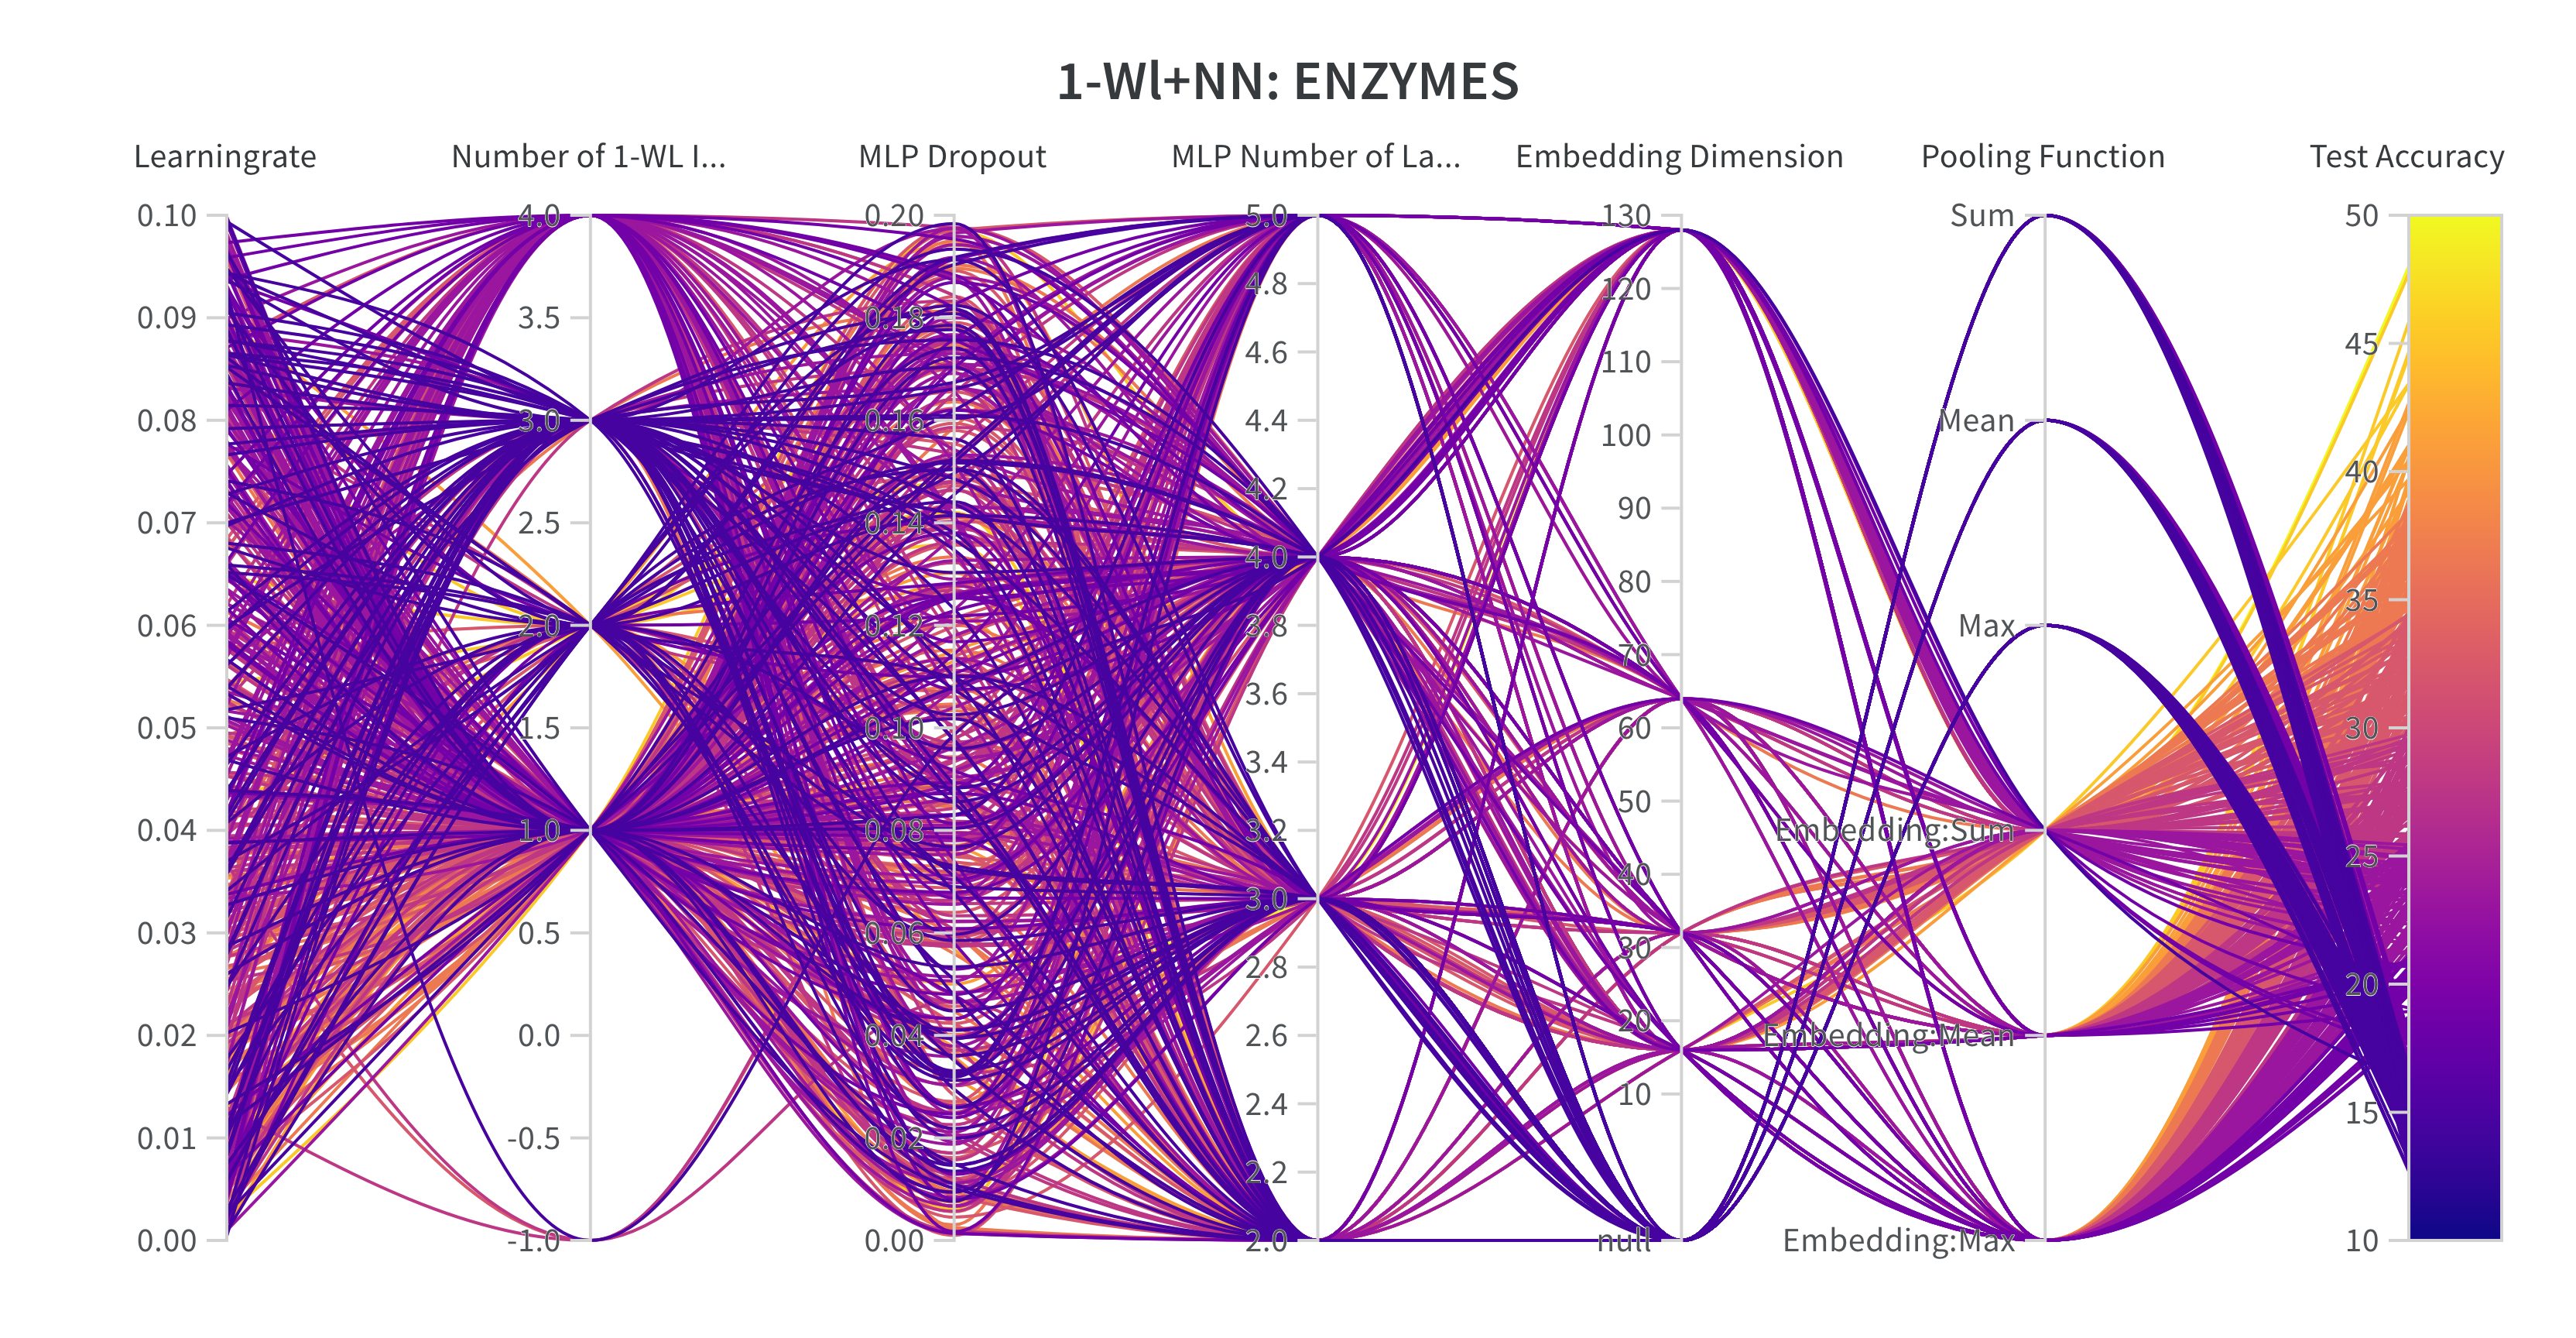
\includegraphics[width=\textwidth]{Figures/hyperparameter_wlnn_enzymes.png}
    \vspace*{-30pt}
    \caption{Overview of the effects of each hyperparameter on the accuracy of the corresponding configured \wlnn model for the \enzymes dataset.}
\end{figure}
\vfill
\begin{figure}[H]
    \centering
    \includegraphics[width=\textwidth]{Figures/hyperparameter_wlnn_imdb.png}
    \caption{Overview of the effects of each hyperparameter on the accuracy of the corresponding configured \wlnn model for the \imdb dataset.}
\end{figure}

\begin{figure}[H]
    \centering
    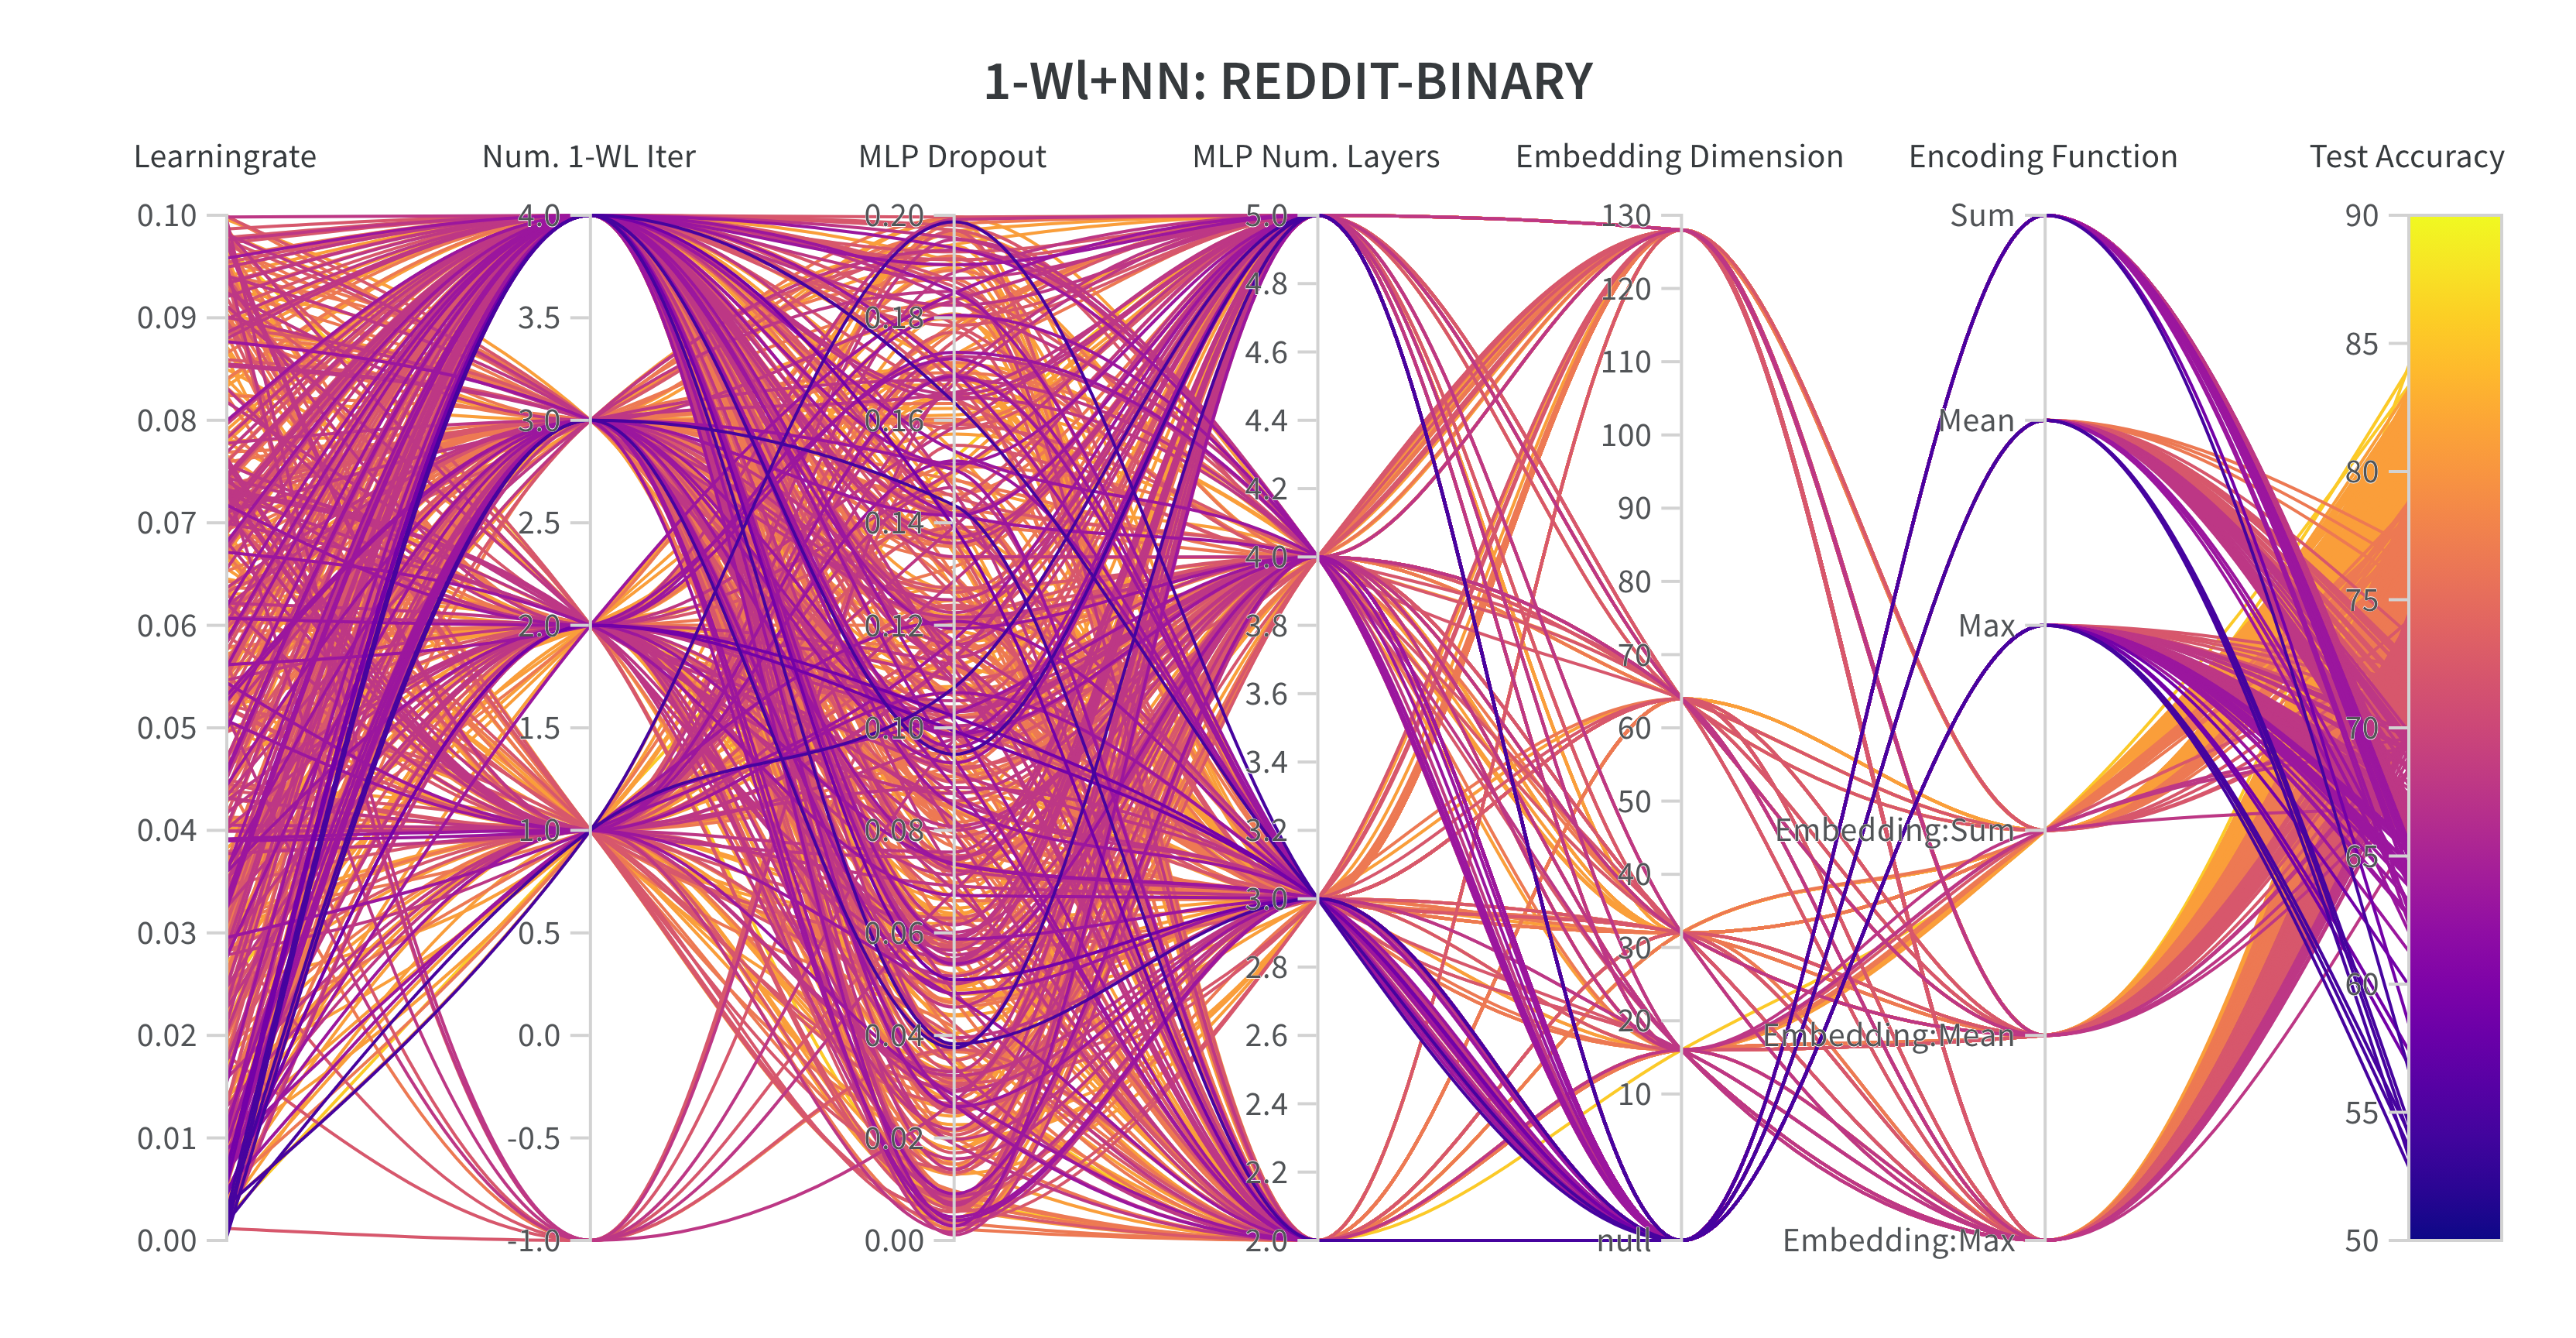
\includegraphics[width=\textwidth]{Figures/hyperparameter_wlnn_mutag.png}
    \vspace*{-30pt}
    \caption{Overview of the effects of each hyperparameter on the accuracy of the corresponding configured \wlnn model for the \mutag dataset.}
\end{figure}
\vfill
\begin{figure}[H]
    \centering
    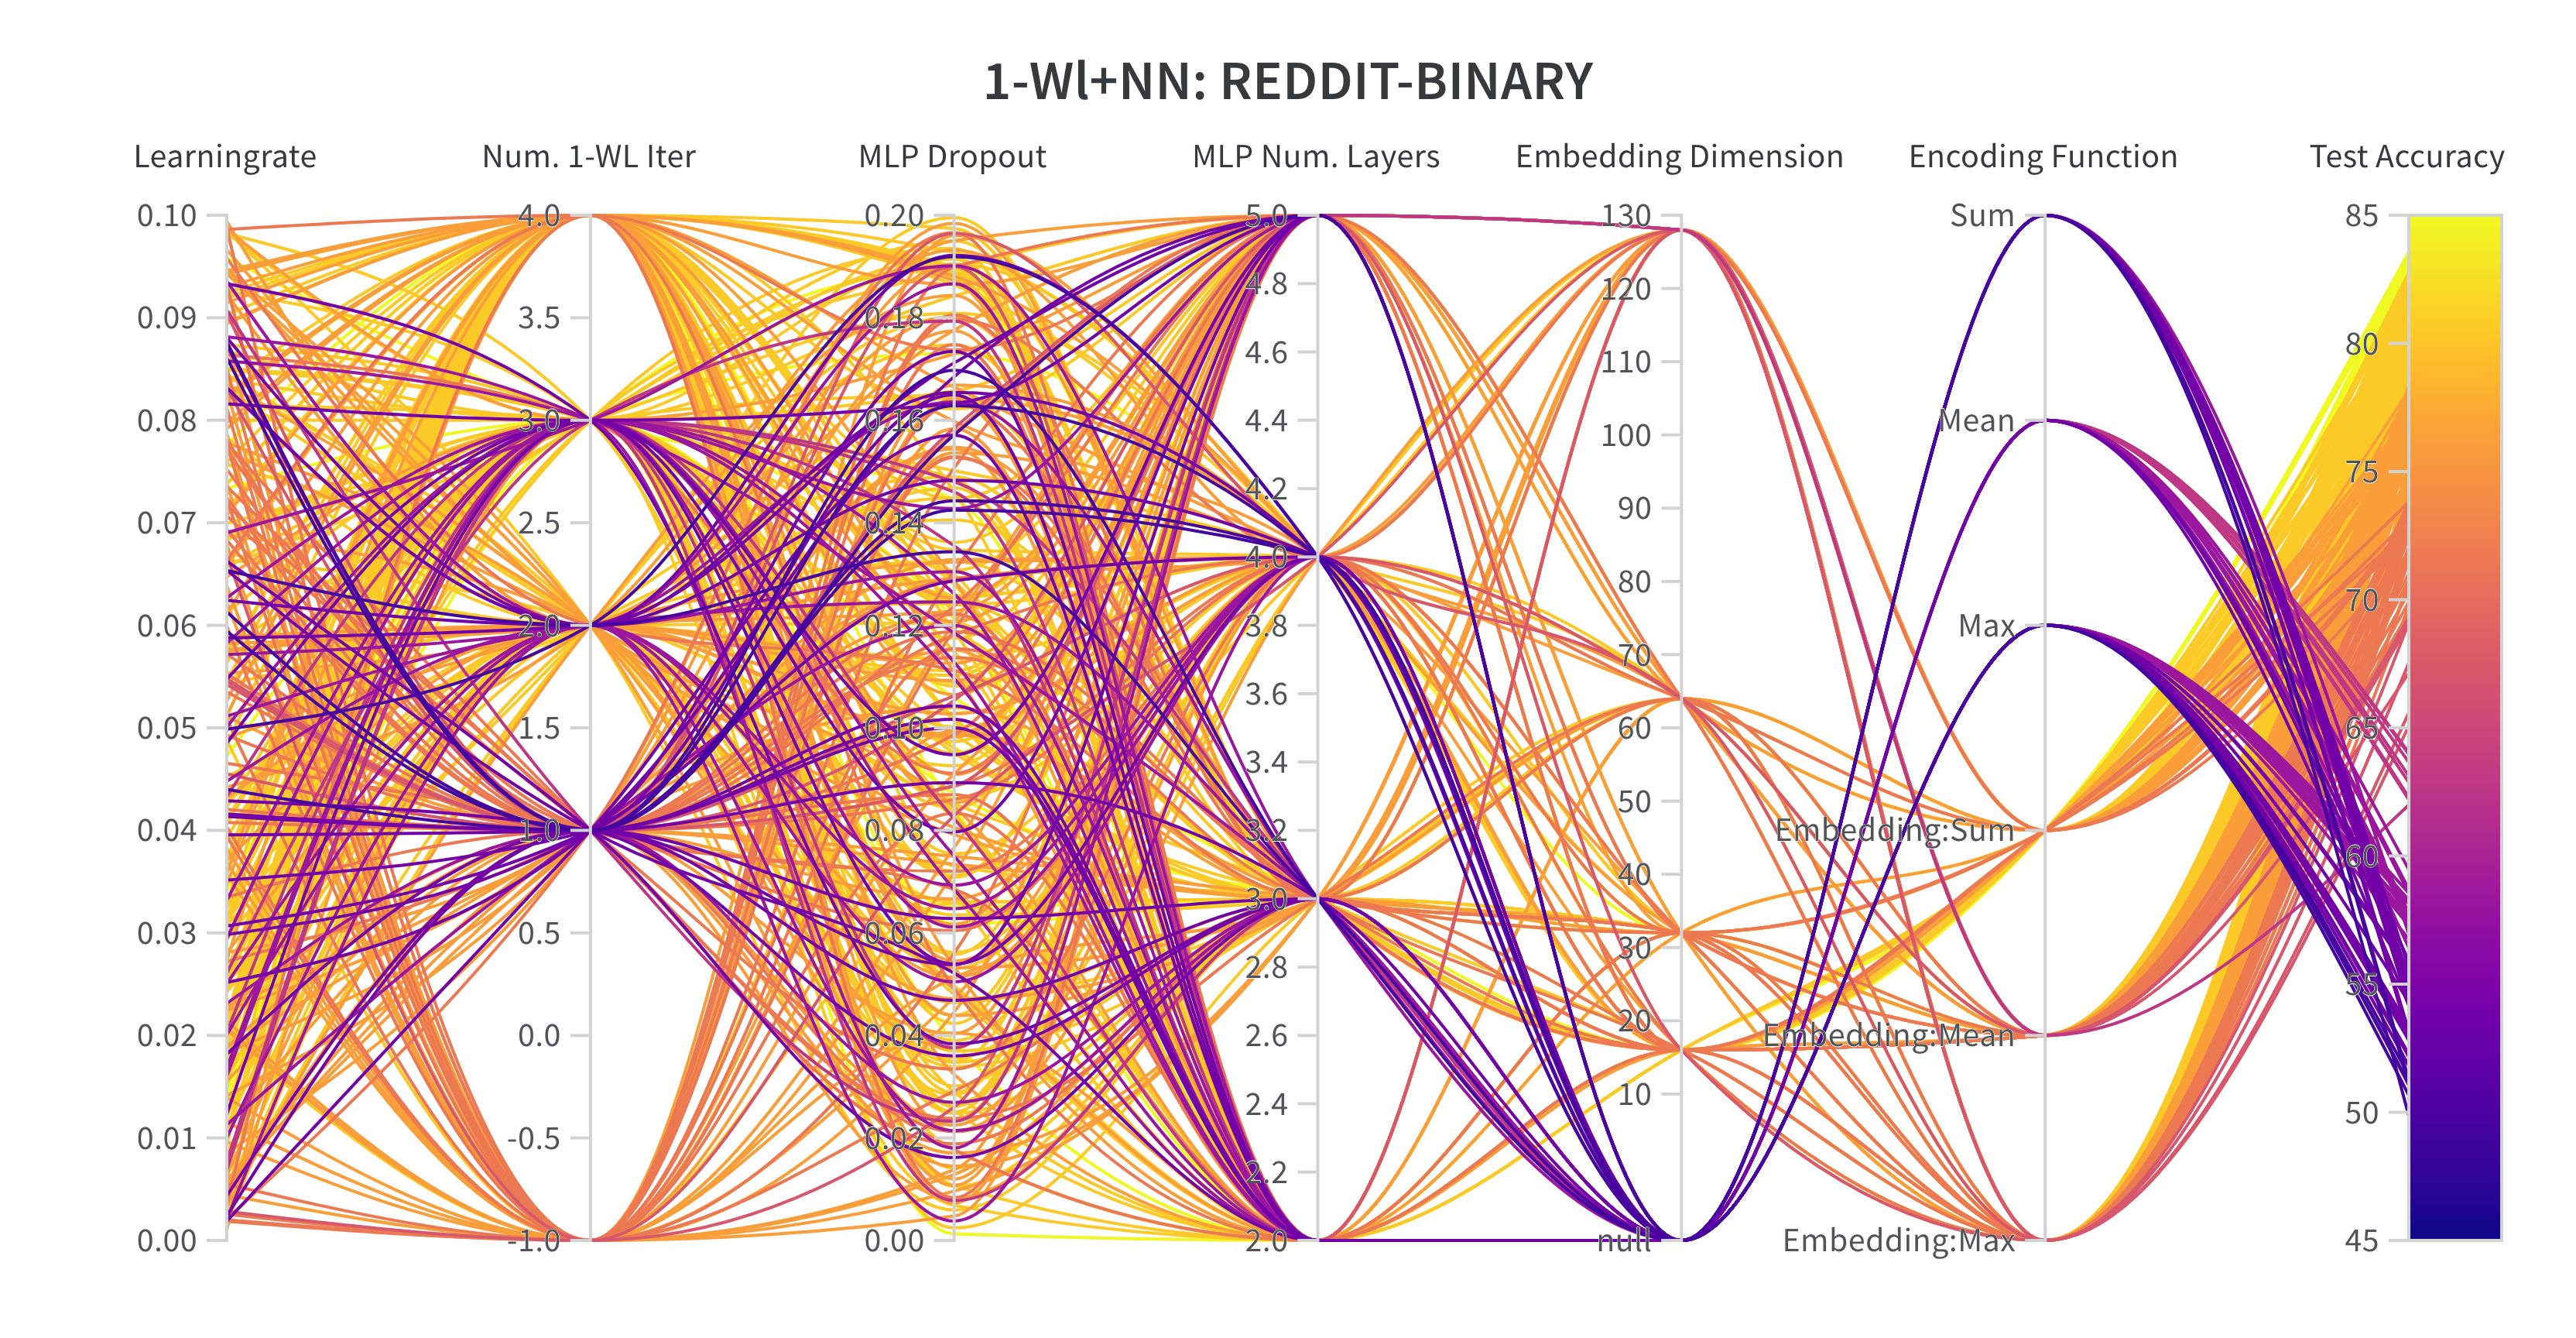
\includegraphics[width=\textwidth]{Figures/hyperparameter_wlnn_nci1.png}
    \vspace*{-30pt}
    \caption{Overview of the effects of each hyperparameter on the accuracy of the corresponding configured \wlnn model for the \nci dataset.}
\end{figure}

\begin{figure}[H]
    \centering
    \includegraphics[width=\textwidth]{Figures/hyperparameter_wlnn_proteins.png}
    \vspace*{-30pt}
    \caption{Overview of the effects of each hyperparameter on the accuracy of the corresponding configured \wlnn model for the \proteins dataset.}
\end{figure}

\begin{figure}[H]
    \centering
    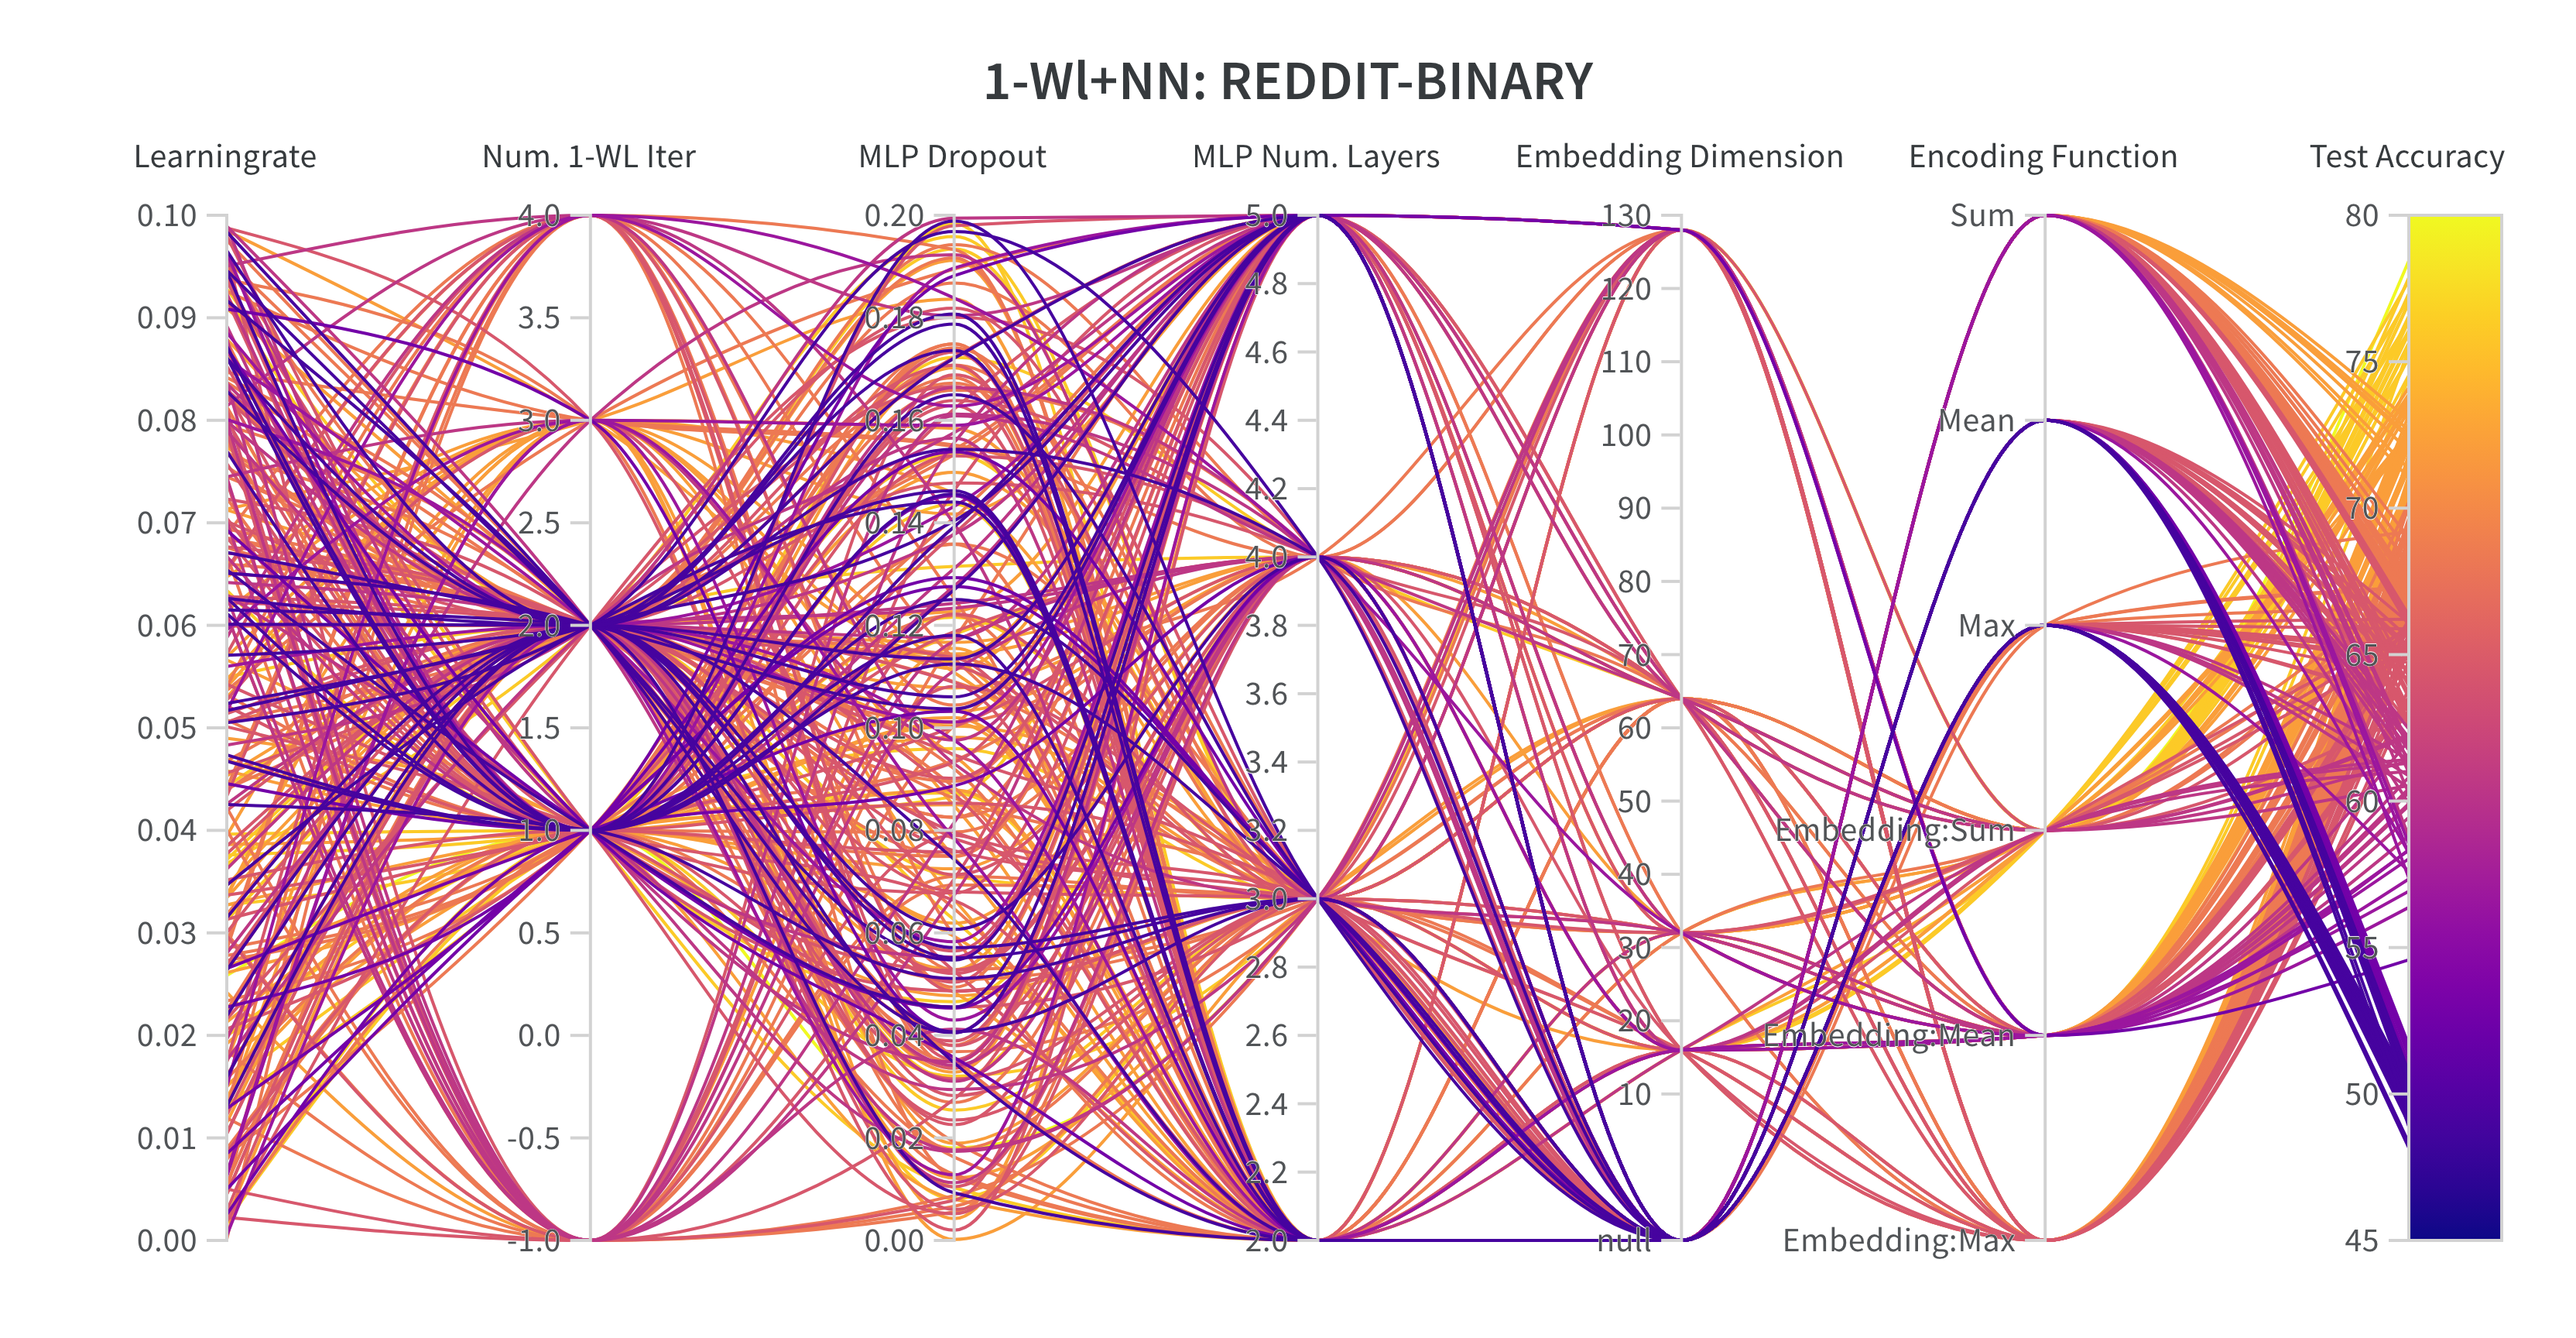
\includegraphics[width=\textwidth]{Figures/hyperparameter_wlnn_reddit.png}
    \vspace*{-30pt}
    \caption{Overview of the effects of each hyperparameter on the accuracy of the corresponding configured \wlnn model for the \reddit dataset.}
\end{figure}


\subsection{Overview of the Impact of each Hyperparameter for \gnn Models}
In this section, we present, similarly to the previous section, the results of our hyperparameter optimization for the \gnn framework on each classification dataset. We plot a random subset of the tested configurations where each line in the visualization represents a single configuration and is color-coded based on its accuracy relative to the other plotted configurations. Bright yellow lines indicate configurations that performed among the best, while dark purple lines represent configurations with the worst performance. The color coding gradually transitions between these two color endpoints, allowing for a clear visual representation of the performance spectrum.

\begin{figure}[H]
    \begin{center}
        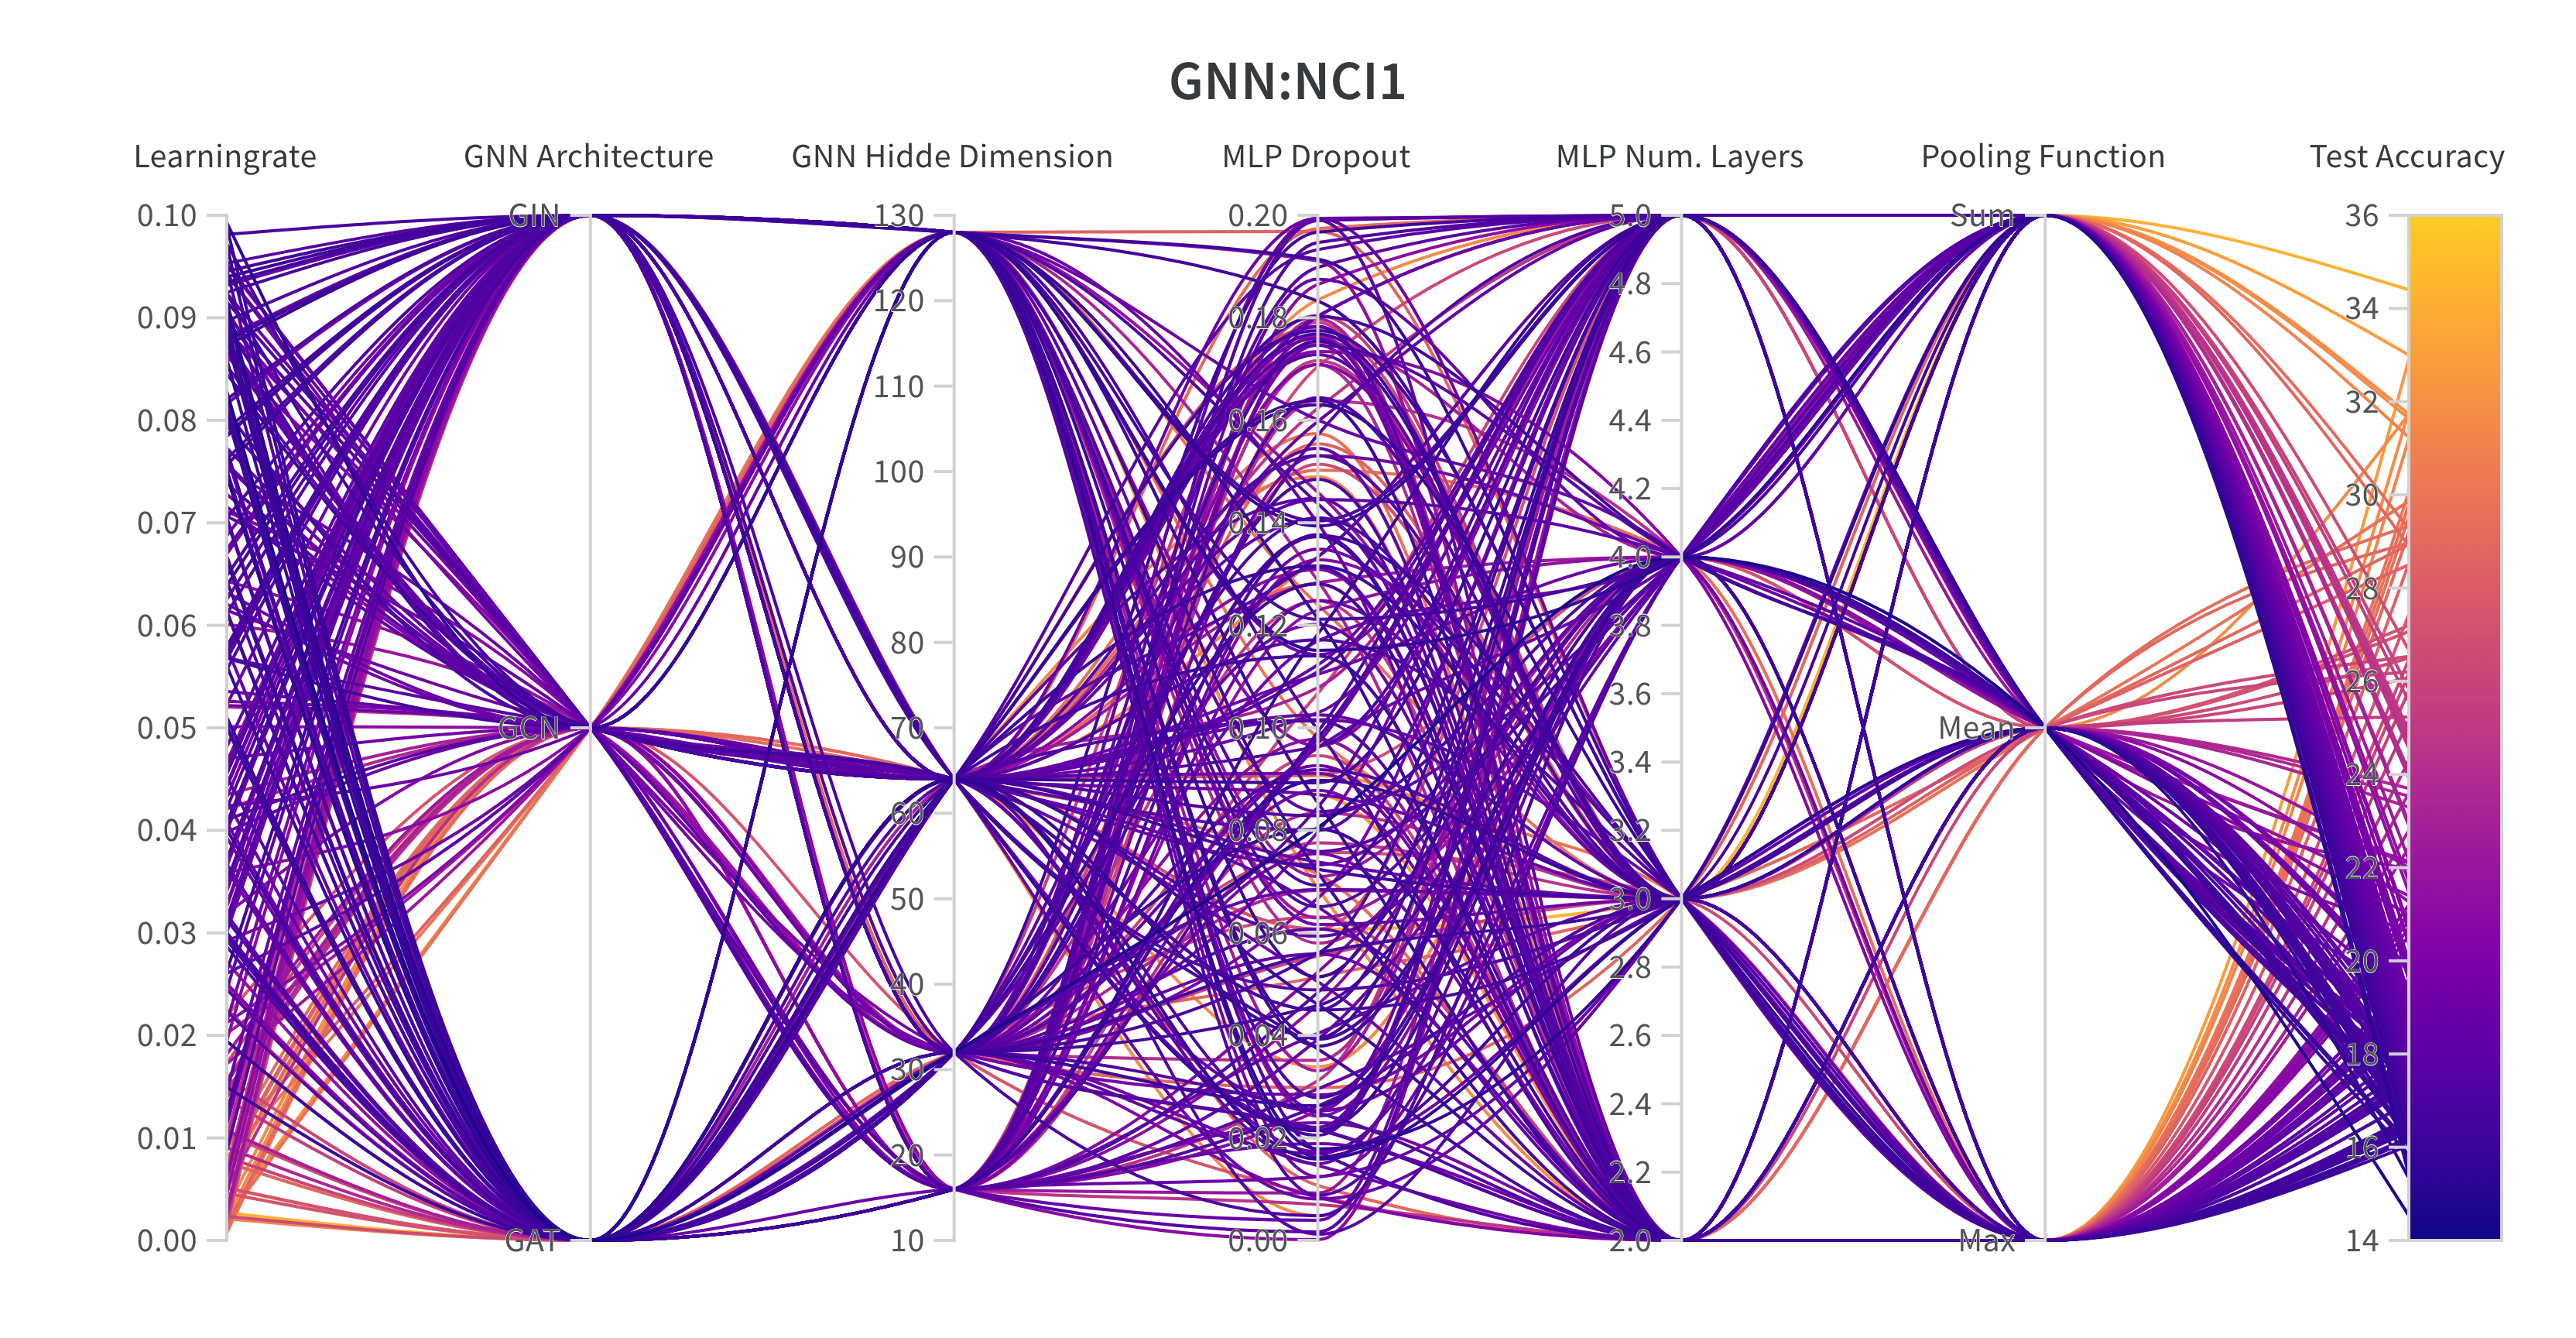
\includegraphics[width=\textwidth]{Figures/hyperparameter_gnn_enzymes.png}
    \end{center}
    \vspace*{-30pt}
    \caption{Overview of the effects of each hyperparameter on the accuracy of the corresponding configured \gnn model for the \enzymes dataset.}
\end{figure}


\begin{figure}[H]
    \centering
    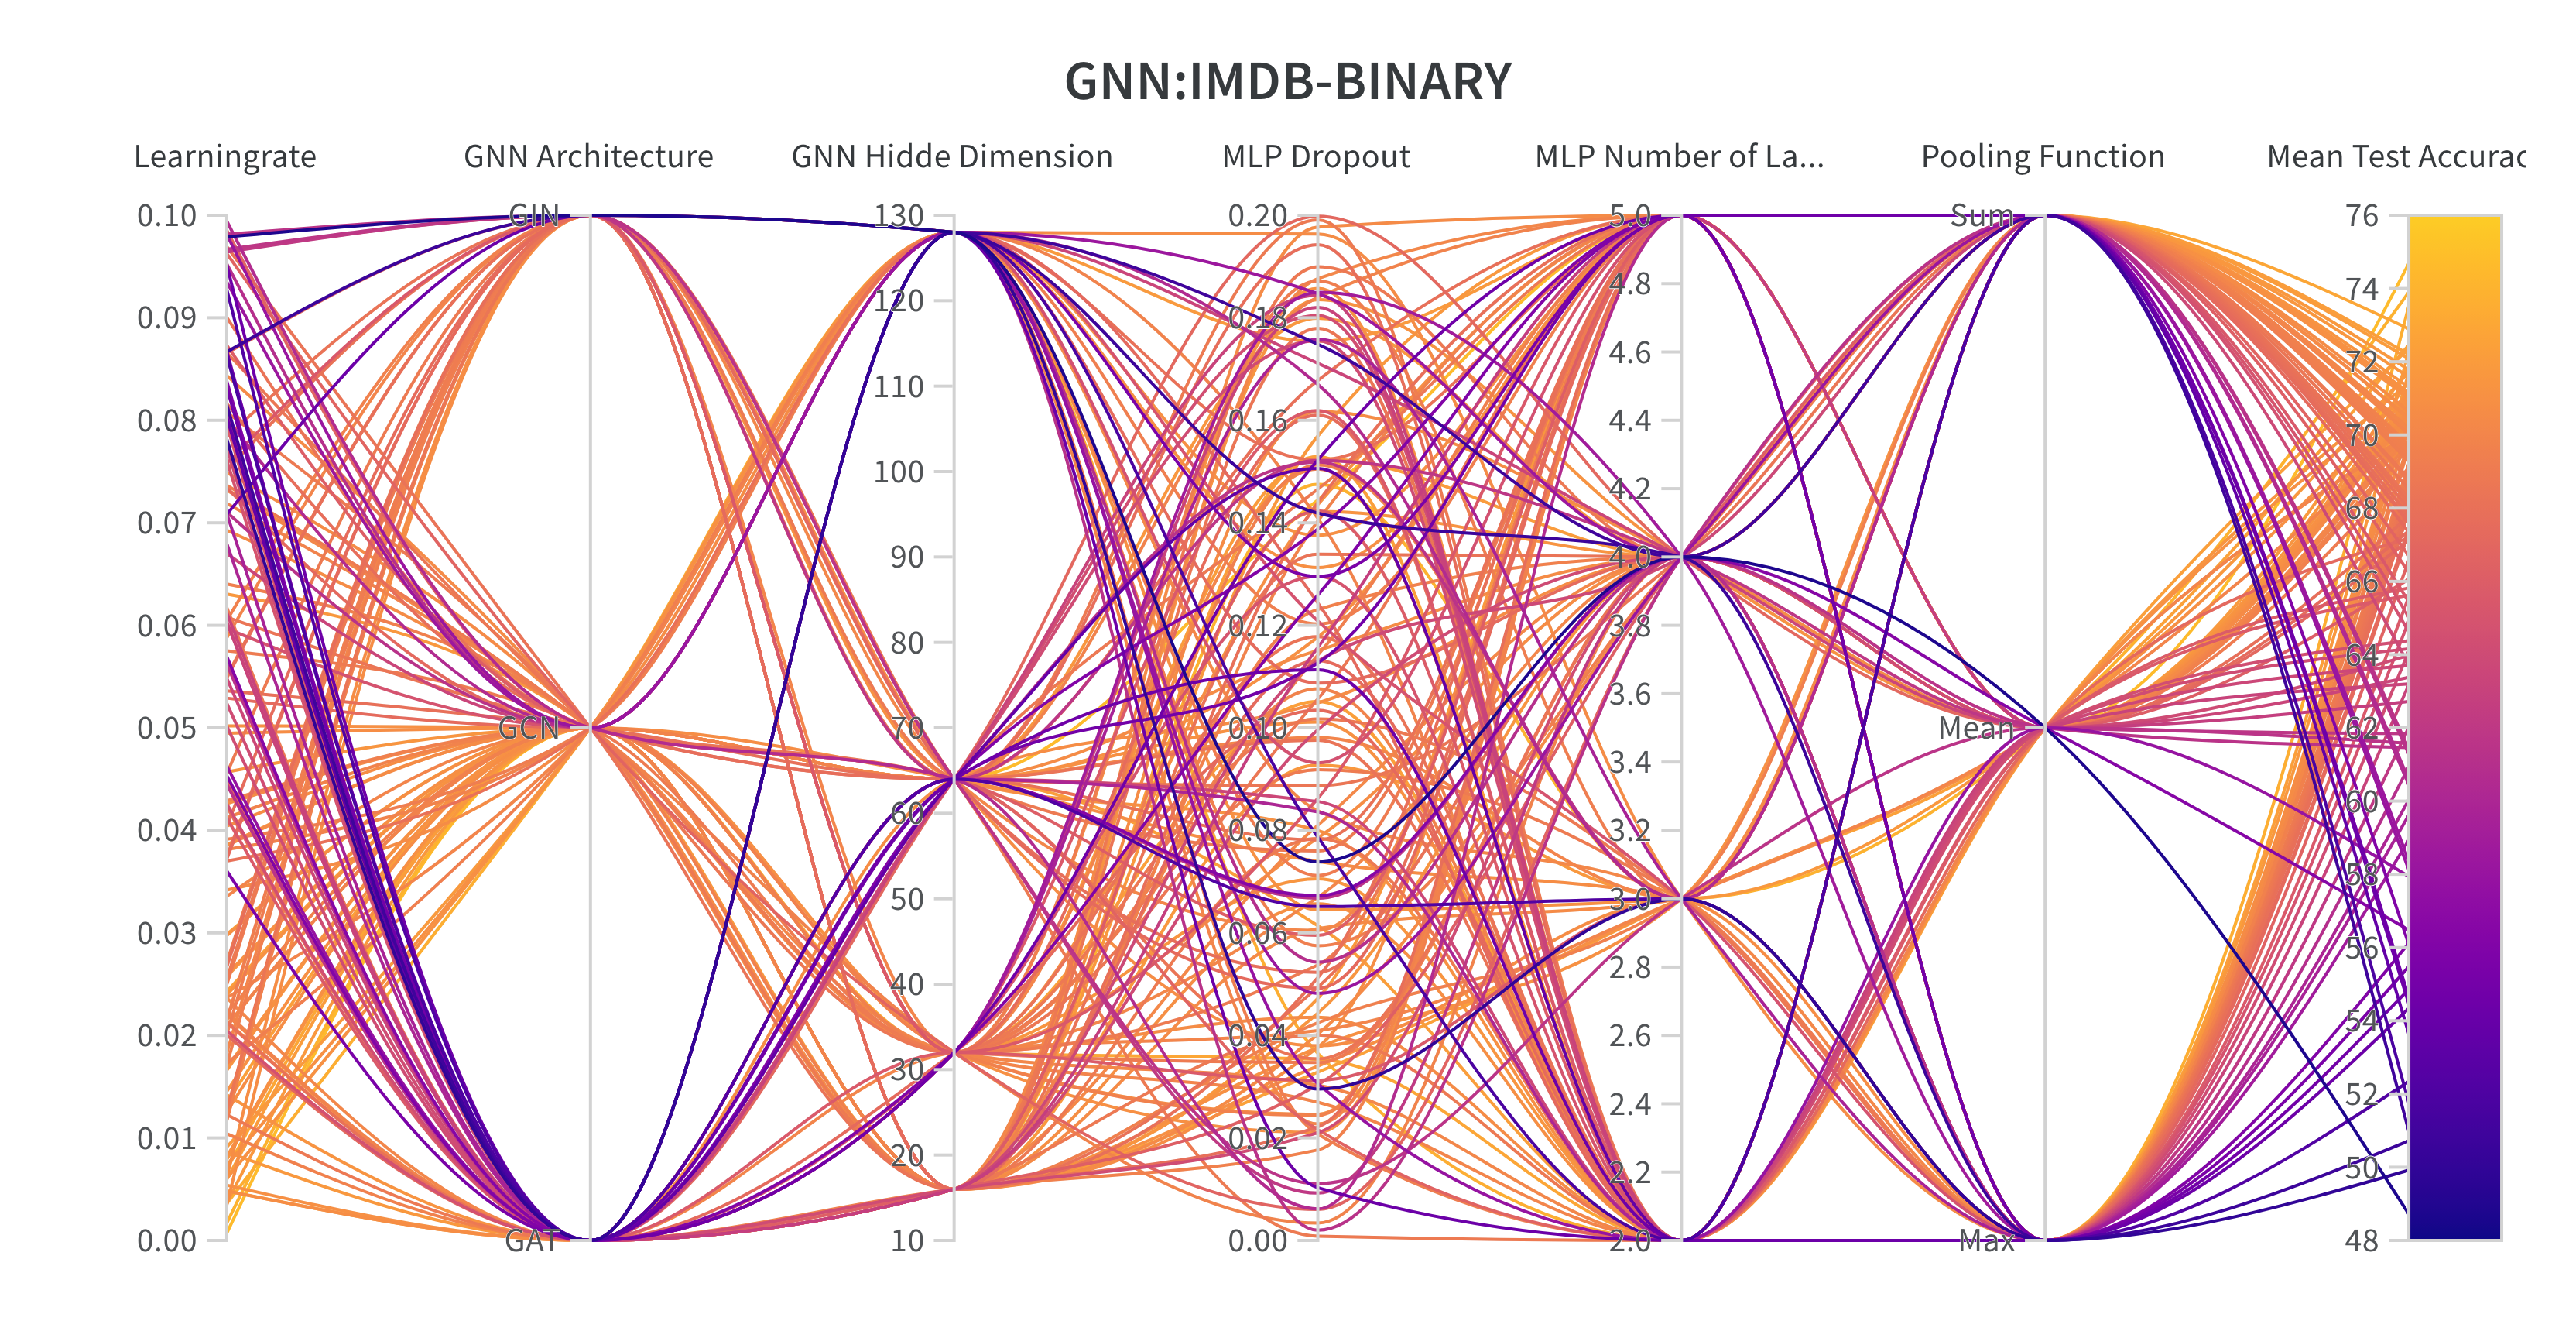
\includegraphics[width=\textwidth]{Figures/hyperparameter_gnn_imdb.png}
    \caption{Overview of the effects of each hyperparameter on the accuracy of the corresponding configured \gnn model for the \imdb dataset.}
\end{figure}

\begin{figure}[H]
    \centering
    \includegraphics[width=\textwidth]{Figures/hyperparameter_gnn_mutag.png}
    \vspace*{-30pt}
    \caption{Overview of the effects of each hyperparameter on the accuracy of the corresponding configured \gnn model for the \mutag dataset.}
\end{figure}

\begin{figure}[H]
    \centering
    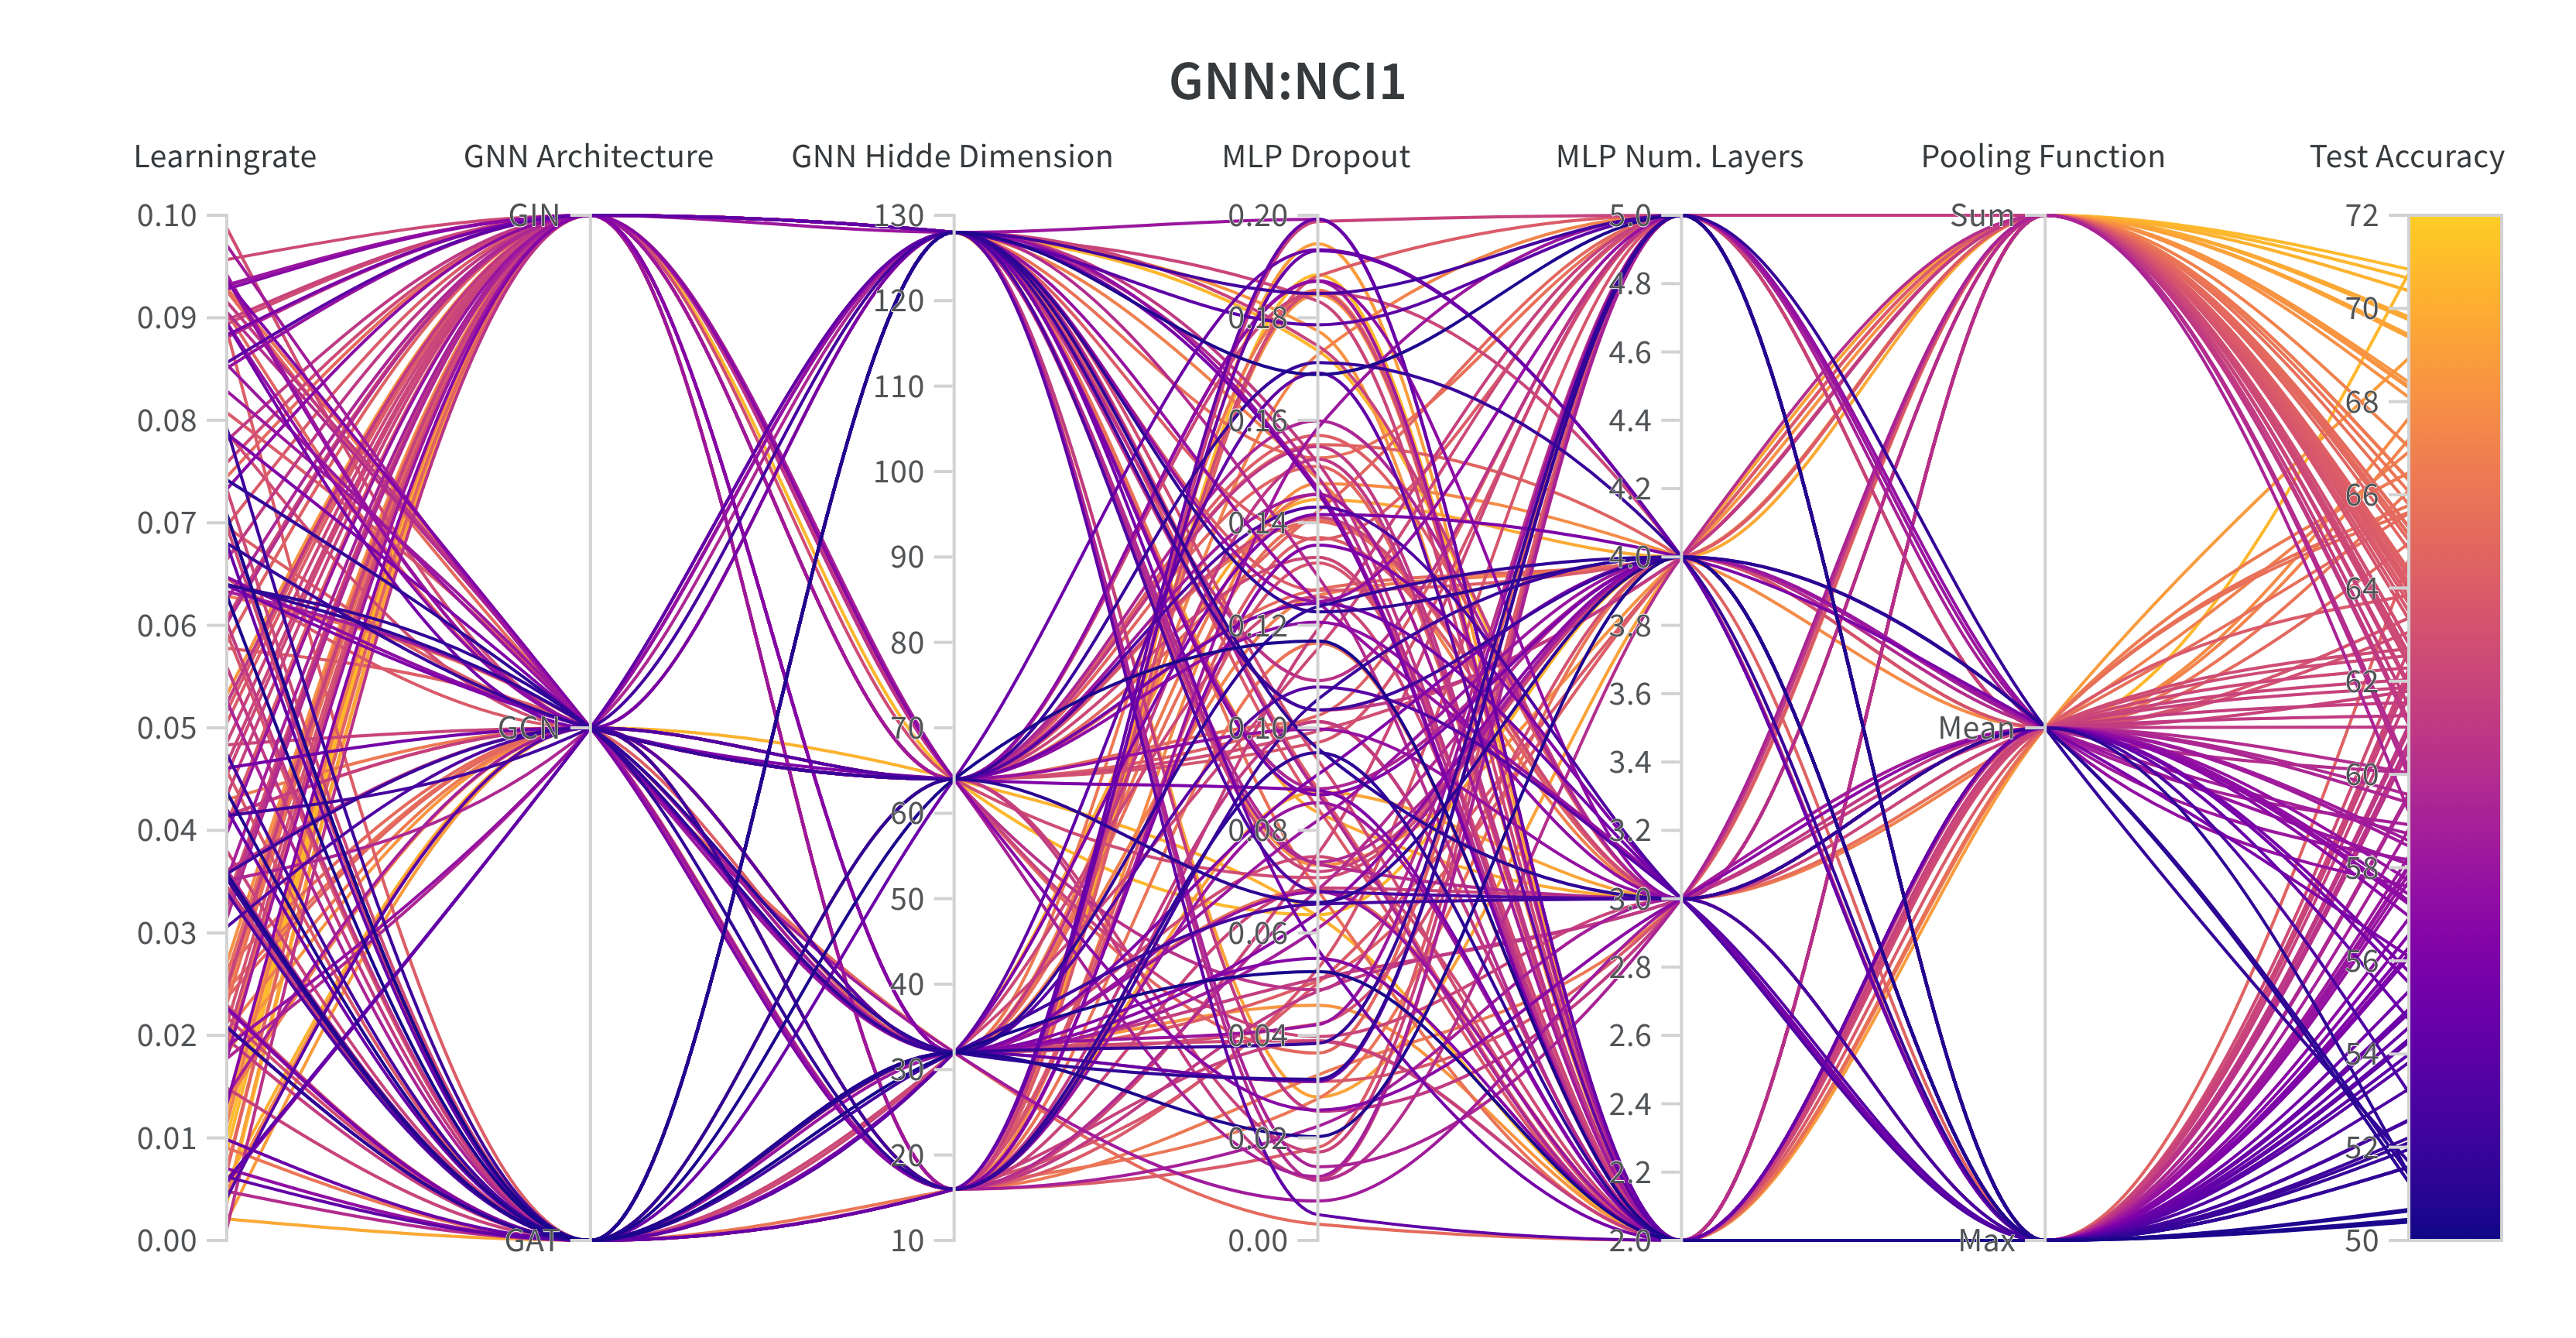
\includegraphics[width=\textwidth]{Figures/hyperparameter_gnn_nci1.png}
    \vspace*{-30pt}
    \caption{Overview of the effects of each hyperparameter on the accuracy of the corresponding configured \gnn model for the \nci dataset.}
\end{figure}

\begin{figure}[H]
    \centering
    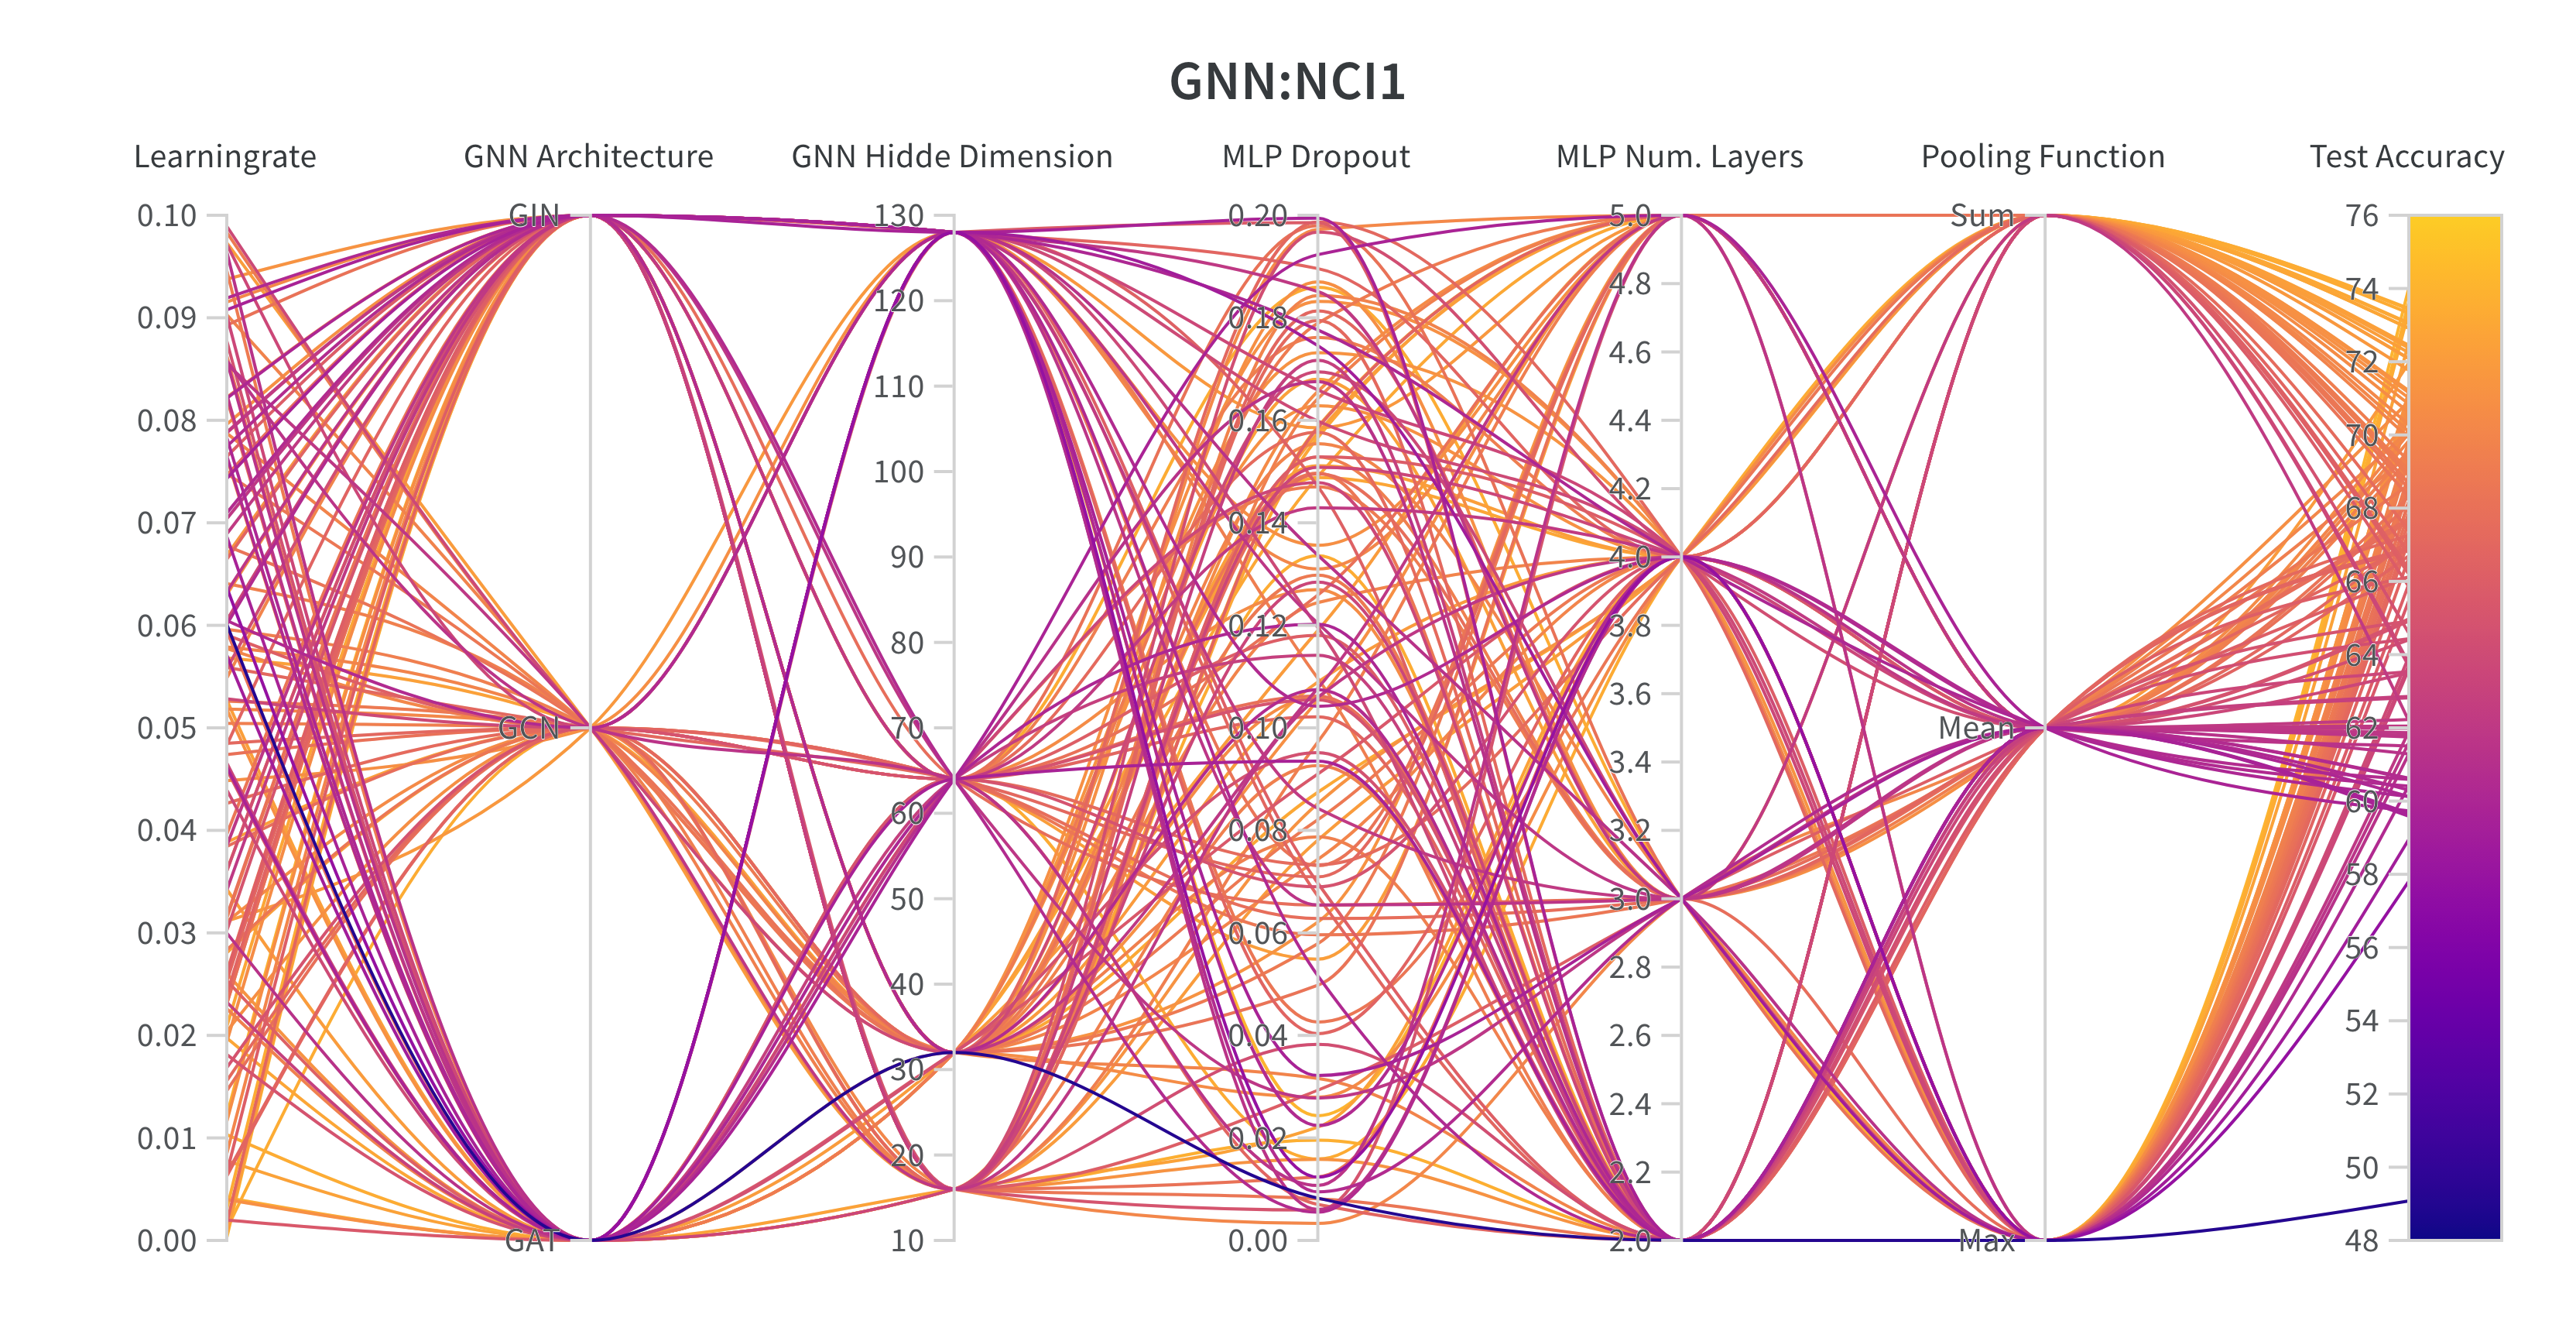
\includegraphics[width=\textwidth]{Figures/hyperparameter_gnn_proteins.png}
    \vspace*{-30pt}
    \caption{Overview of the effects of each hyperparameter on the accuracy of the corresponding configured \gnn model for the \proteins dataset.}
\end{figure}

\begin{figure}[H]
    \centering
    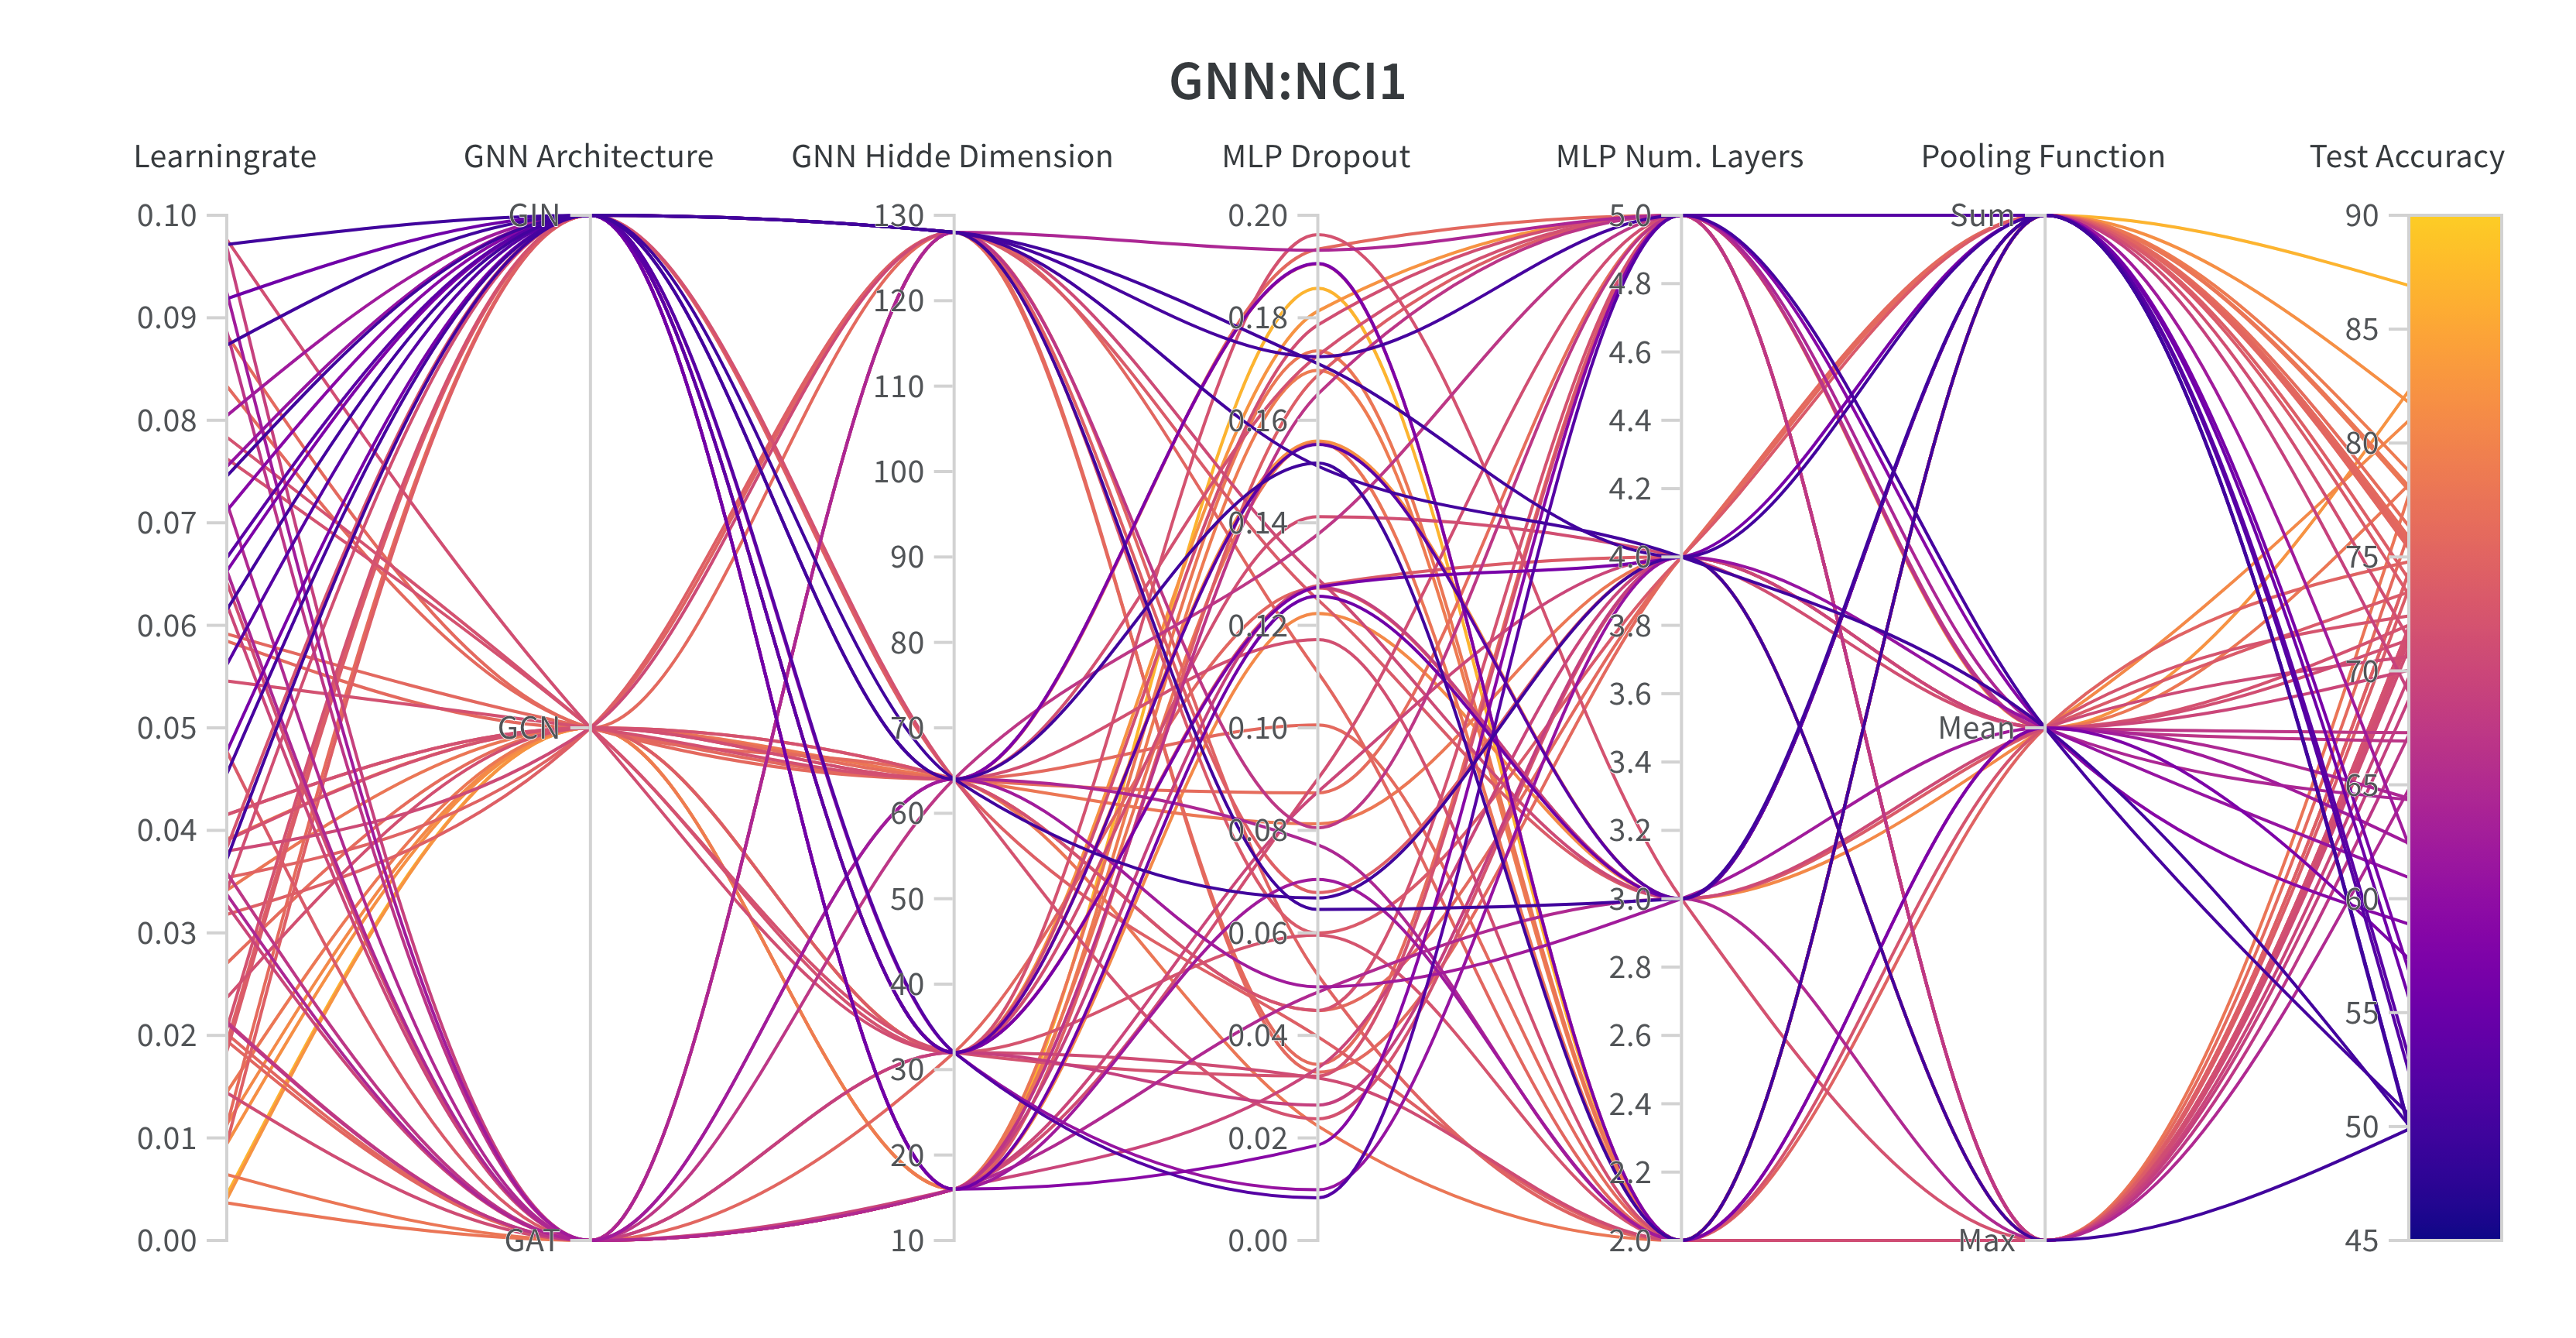
\includegraphics[width=\textwidth]{Figures/hyperparameter_gnn_reddit.png}
    \vspace*{-30pt}
    \caption{Overview of the effects of each hyperparameter on the accuracy of the corresponding configured \gnn model for the \reddit dataset.}
\end{figure}

\subsection{Overview of the Number of Configurations}
\begin{table}[H]
	\caption{Overview of the number of different configurations tested for each model type and each dataset.}
	\label{tab:num_runs}
    \resizebox{.975\textwidth}{!}{ 	\renewcommand{\arraystretch}{1.05}
		\begin{tabular}{@{}c <{\enspace}@{}lcccccccccc}	\toprule
			& \multirow{3}{*}{\vspace*{4pt}\textbf{Method}}&\multicolumn{10}{c}{\textbf{Dataset}}\\\cmidrule{3-12}
            & & \multicolumn{6}{c}{\textbf{Classification}} & \multicolumn{4}{c}{\textbf{Regression}}\\\cmidrule(lr){3-8}\cmidrule(lr){9-12}
			& & \enzymes & \imdb & \mutag & \nci & \proteins & \reddit & \alchemy & \alchemyten & \zinc & \zincten
			\\
			\toprule
			\multirow[c]{7}{*}{\rotatebox{90}{\wlnn}} 	&
			\textsf{Max} & 86 & 70 & 150 & 26 & 35 & 40 & 0 & 0 & 0 & 0 \\
			& \textsf{Mean} & 76 & 67 & 120 & 19 & 27 & 40 & 0 & 0 & 0 & 0 \\
			& \textsf{Sum} &  85 & 67 & 130 & 14 & 29 & 41 & 0 & 0 & 0 & 0 \\  
			\cmidrule{2-12}  		
			& \textsf{Embedding-Max} & 338 & 282 & 290 & 79 & 245 & 45 & 3 & 95 & 6 & 33 \\
			& \textsf{Embedding-Mean} & 288 & 271 & 299 & 109 & 216 & 50 & 6 & 77 & 8 & 24 \\ 
			& \textsf{Embedding-Sum} & 296 & 293 & 302 & 79 & 215 & 48 & 5 & 273 & 7 & 18 \\ 
			\cmidrule{1-12}
			\multirow[c]{10}{*}{\rotatebox{90}{Graph Neural Networks}} 
			& \textsf{GAT:Max} & 17 & 17 & 36 & 11 & 10 & 6 & 0 & 0 & 0 & 0 \\
			& \textsf{GAT:Mean} & 28 & 15 & 29 & 12 & 10 & 6 & 0 & 0 & 0 & 0 \\
			& \textsf{GAT:Sum} & 26 & 17 & 37 & 15 & 16 & 6 & 0 & 0 & 0 & 0 \\
			\cmidrule{2-12}
			& \textsf{GCN:Max} & 31 & 22 & 37 & 17 & 10 & 9 & 0 & 0 & 0 & 0 \\
			& \textsf{GCN:Mean} & 19 & 26 & 26 & 19 & 16 & 5 & 0 & 0 & 0 & 0 \\
			& \textsf{GCN:Sum} & 30 & 29 & 27 & 17 & 14 & 10 & 0 & 0 & 0 & 0 \\  
			\cmidrule{2-12}	
			& \textsf{GIN:Max} & 21 & 17 & 28 & 25 & 20 & 3 & 1 & 1 & 1 & 1 \\
			& \textsf{GIN:Mean} & 31 & 9 & 31 & 18 & 26 & 9 & 2 & 2 & 2 & 2 \\
			& \textsf{GIN:Sum} & 26 & 9 & 36 & 20 & 11 & 9 & 1 & 1 & 1 & 1 \\
            \cmidrule{1-12}
            \multirow[c]{10}{*}{\rotatebox{90}{\wl:\gnn}} 
			& \textsf{GAT:Max} & 2 & 4 & 1 & 9 & 4 & 2 & 0 & 0 & 0 & 0 \\
			& \textsf{GAT:Mean} & 3 & 4 & 6 & 6 & 7 & 4 & 0 & 0 & 0 & 0 \\
			& \textsf{GAT:Sum} & 5 & 5 & 6 & 9 & 4 & 4 & 0 & 0 & 0 & 0 \\
			\cmidrule{2-12}
			& \textsf{GCN:Max} & 2 & 6 & 4 & 12 & 6 & 3 & 0 & 0 & 0 & 0 \\
			& \textsf{GCN:Mean} & 3 & 5 & 3 & 10 & 8 & 2 & 0 & 0 & 0 & 0 \\
			& \textsf{GCN:Sum} & 6 & 2 & 3 & 5 & 5 & 3 & 0 & 0 & 0 & 0 \\
			\cmidrule{2-12}	
			& \textsf{GIN:Max} & 3 & 4 & 4 & 9 & 7 & 5 & 0 & 0 & 0 & 0 \\
			& \textsf{GIN:Mean} & 2 & 6 & 2 & 10 & 7 & 3 & 0 & 0 & 0 & 0 \\
			& \textsf{GIN:Sum} & 4 & 2 & 4 & 11 & 4 & 4 & 0 & 0 & 0 & 0 \\
			\bottomrule
		\end{tabular}}            
\end{table}



\section{Empirical Testing}
\subsection{Approximating \wl Coloring: Investigating \gnn Node Representations}

\begin{table}[H]
    \caption{Overview of the number of unique colors in the colorings computed by the \wl algorithm when applied to each dataset. Specifically, we specified the number of iterations of the \wl algorithm. Additionally, the ``\# Nodes'' column showcases the maximum number of unique colors that can be appear in the colorings.}
    \label{tab:unique_colors}
    \centering
    \resizebox{\textwidth}{!}{ 	\renewcommand{\arraystretch}{0.9}
    \begin{tabular}{@{}c <{\enspace}@{}lrrrrrrrrrrr | r}
    \toprule
        & \multirow{3}{*}{\vspace*{4pt}\textbf{Dataset}}&\multicolumn{11}{c}{\textbf{Number of \wl Iterations}}\\\cmidrule{3-14}
        & & 0 & 1 & 2 & 3 & 4 & 5 & 6 & 7 & 8 & 9 & 10 & \# Nodes\\
        \midrule
        \multirow{6}{*}{\rotatebox{90}{Classification}}
        & \enzymes & 2 & 231 & 10\,416 & 15\,208 & 16\,029 & 16\,450 & 16\,722 & 16\,895 & 17\,026 & 17\,130 & 17\,204 & 195\,80\\
        & \imdb & 1 & 65 & 2\,931 & 3\,595 & 3\,595 & 3\,595 & 3\,595 & 3\,595 & 3\,595 & 3\,595 & 3\,595 & 19\,773 \\
        & \mutag & 2 & 33 & 174 & 572 & 1\,197 & 1\,766 & 2\,167 & 2\,403 & 2\,511 & 2\,560 & 2\,579 & 3\,371 \\
        & \nci & 2 & 292 & 4\,058 & 22\,948 & 44\,508 & 58\,948 & 68\,632 & 75\,754 & 81\,263 & 85\,590 & 88\,968 & 122\,747\\
        & \proteins & 2 & 297 & 20\,962 & 35\,676 & 37\,940 & 38\,653 & 38\,926 & 39\,064 & 39\,141 & 39\,180 & 39\,203 & 43\,471\\
        & \reddit & 1 & 566 & 71\,893 & 244\,529 & 317\,728 & 333\,258 & 335\,961 & 336\,412 & 336\,490 & 336\,506 & 336\,507 & 859\,254 \\
        \cmidrule{2-14}
        \multirow{4}{*}{\rotatebox{90}{Regress.}}
        & \alchemy & 2 & 70 & 4\,782 & 164\,224 & 620\,332 & 995\,264 & 1\,166\,951 & 1\,216\,094 & 1\,225\,861 & 1\,227\,632 & 1\,227\,904 & 2\,046\,329\\
        & \alchemyten & 2 & 70 & 2\,764 & 33\,903 & 76\,822 & 98\,394 & 104\,687 & 105\,907 & 106\,109 & 106\,149 & 106\,166 & 121\,422\\
        & \zinc & 2 & 773 & 288\,74 & 290\,473 & 1\,000\,917 & 1\,977\,437 & 2\,921\,087 & 3\,690\,341 & 4\,270\,959 & 4\,681\,881 & 4\,945\,363 & 5\,775\,257 \\
        & \zincten & 2 & 392 & 9\,818 & 61\,198 & 132\,862 & 185\,699 & 216\,210 & 233\,484 & 242\,866 & 247\,688 & 249\,971 & 278\,179 \\
        \bottomrule
    \end{tabular}}
\end{table}

\begin{figure}[!ht]
    \centering
    \begin{minipage}[b]{0.45992852703\textwidth}
        \centering
        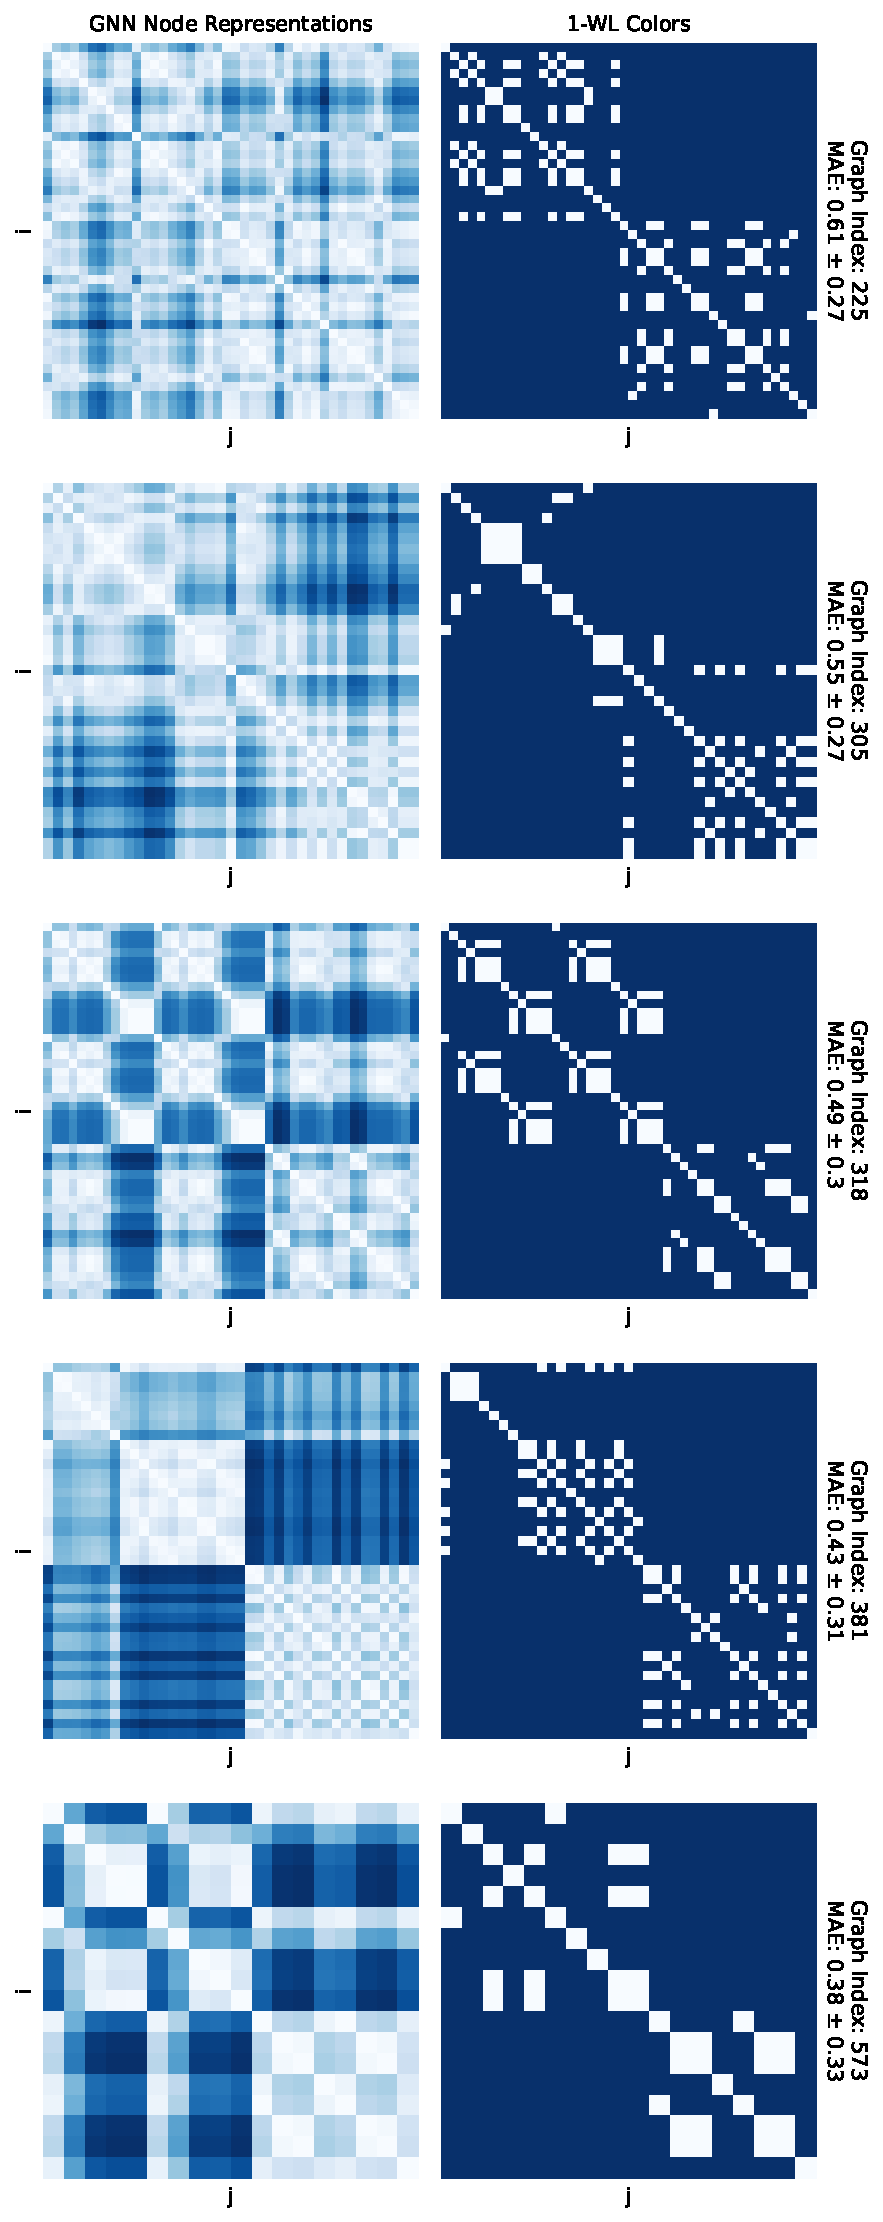
\includegraphics[width=\textwidth, left]{Figures/heatmaps_ENZYMES_0.pdf}
    \end{minipage}
    \hfill
    \begin{minipage}[b]{0.53007147296\textwidth}
        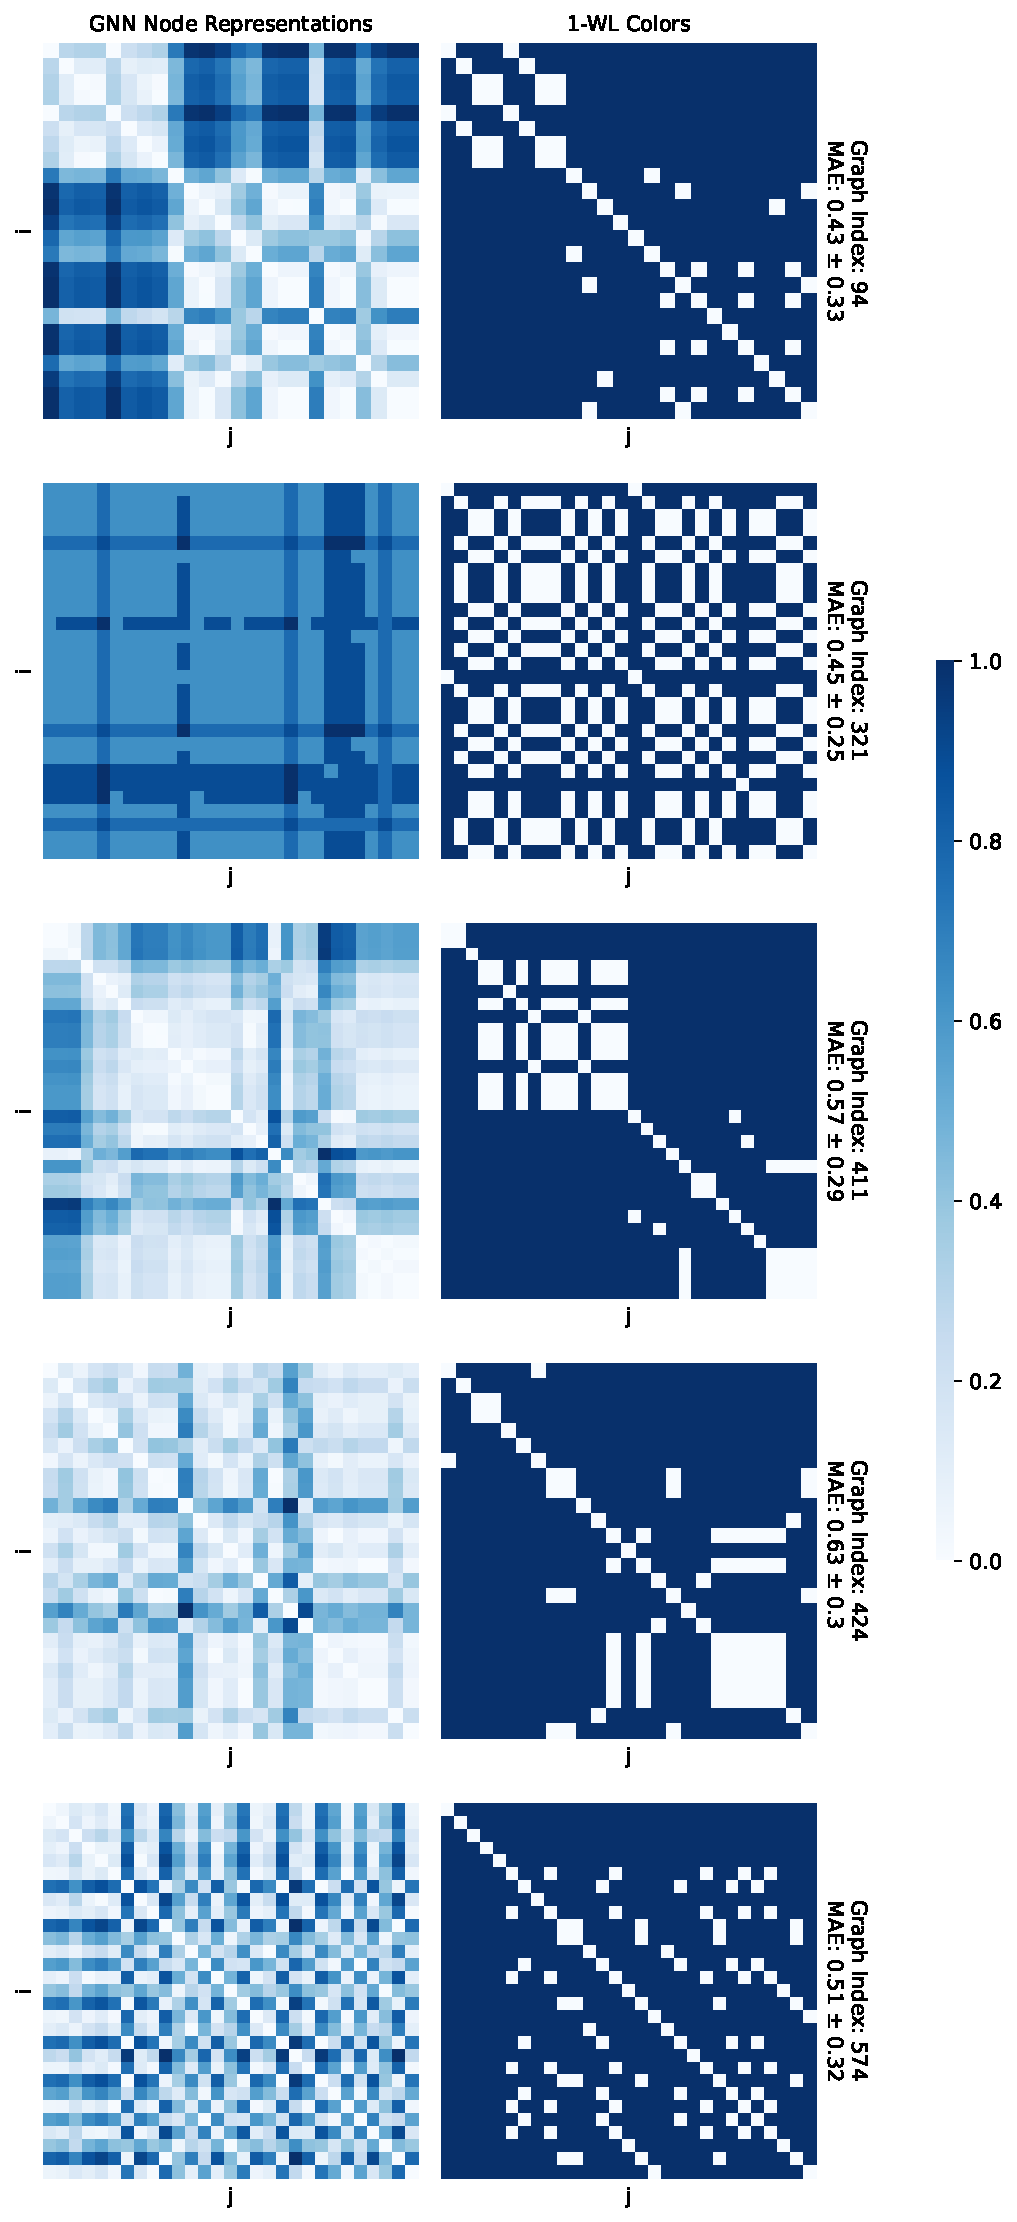
\includegraphics[width=\textwidth, right]{Figures/heatmaps_ENZYMES_1.pdf}
    \end{minipage}
    \hfill
    \caption{Visualizing the performance of the best performing GNN on the \textsc{Enzymes} dataset in approximating node colors computed by the 1-WL algorithm. The ten graphs shown are randomly sampled from the GNN's test set, and the 1-WL algorithm ran only for one iteration. The average error for the entire test set is $0.49 \pm 0.3$.}
    \label{fig:gnn_approx_enzymes}
\end{figure}

\begin{figure}[!ht]
    \centering
    \begin{minipage}[b]{0.45992852703\textwidth}
        \centering
        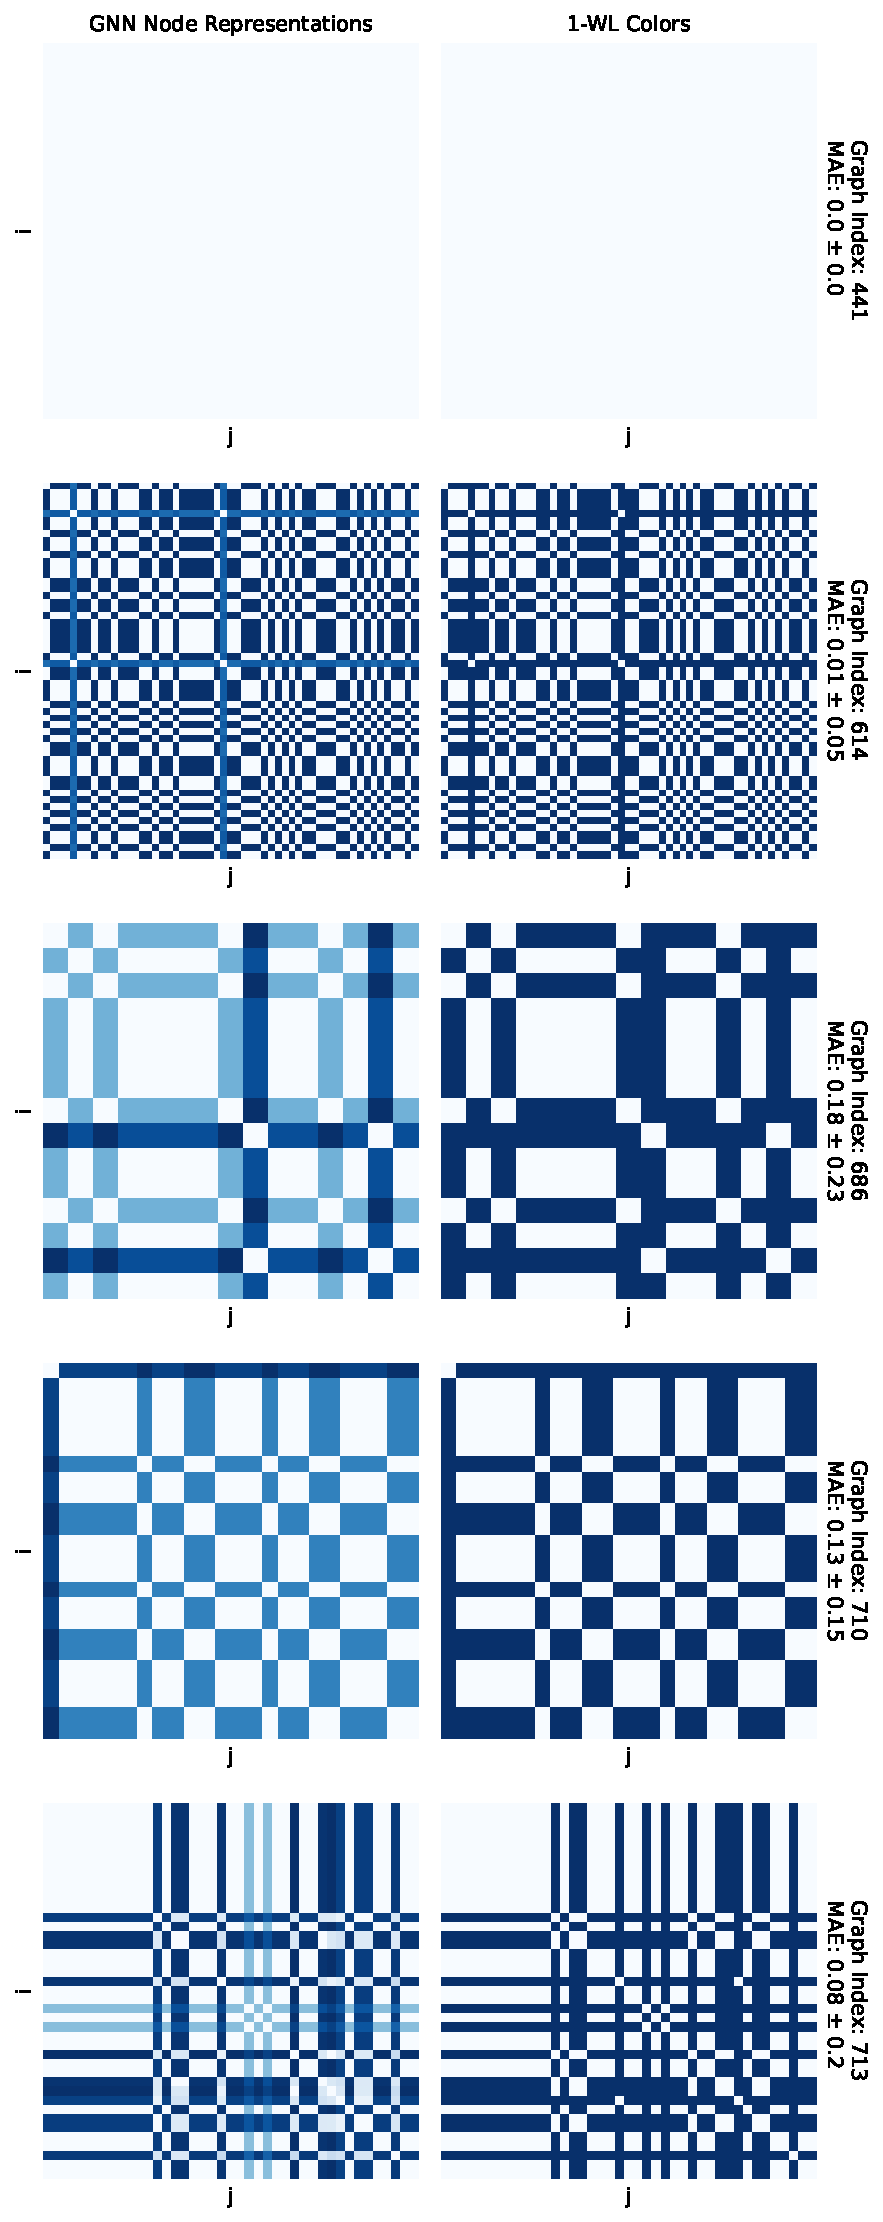
\includegraphics[width=\textwidth, left]{Figures/heatmaps_IMDB-BINARY_0.pdf}
    \end{minipage}
    \hfill
    \begin{minipage}[b]{0.53007147296\textwidth}
        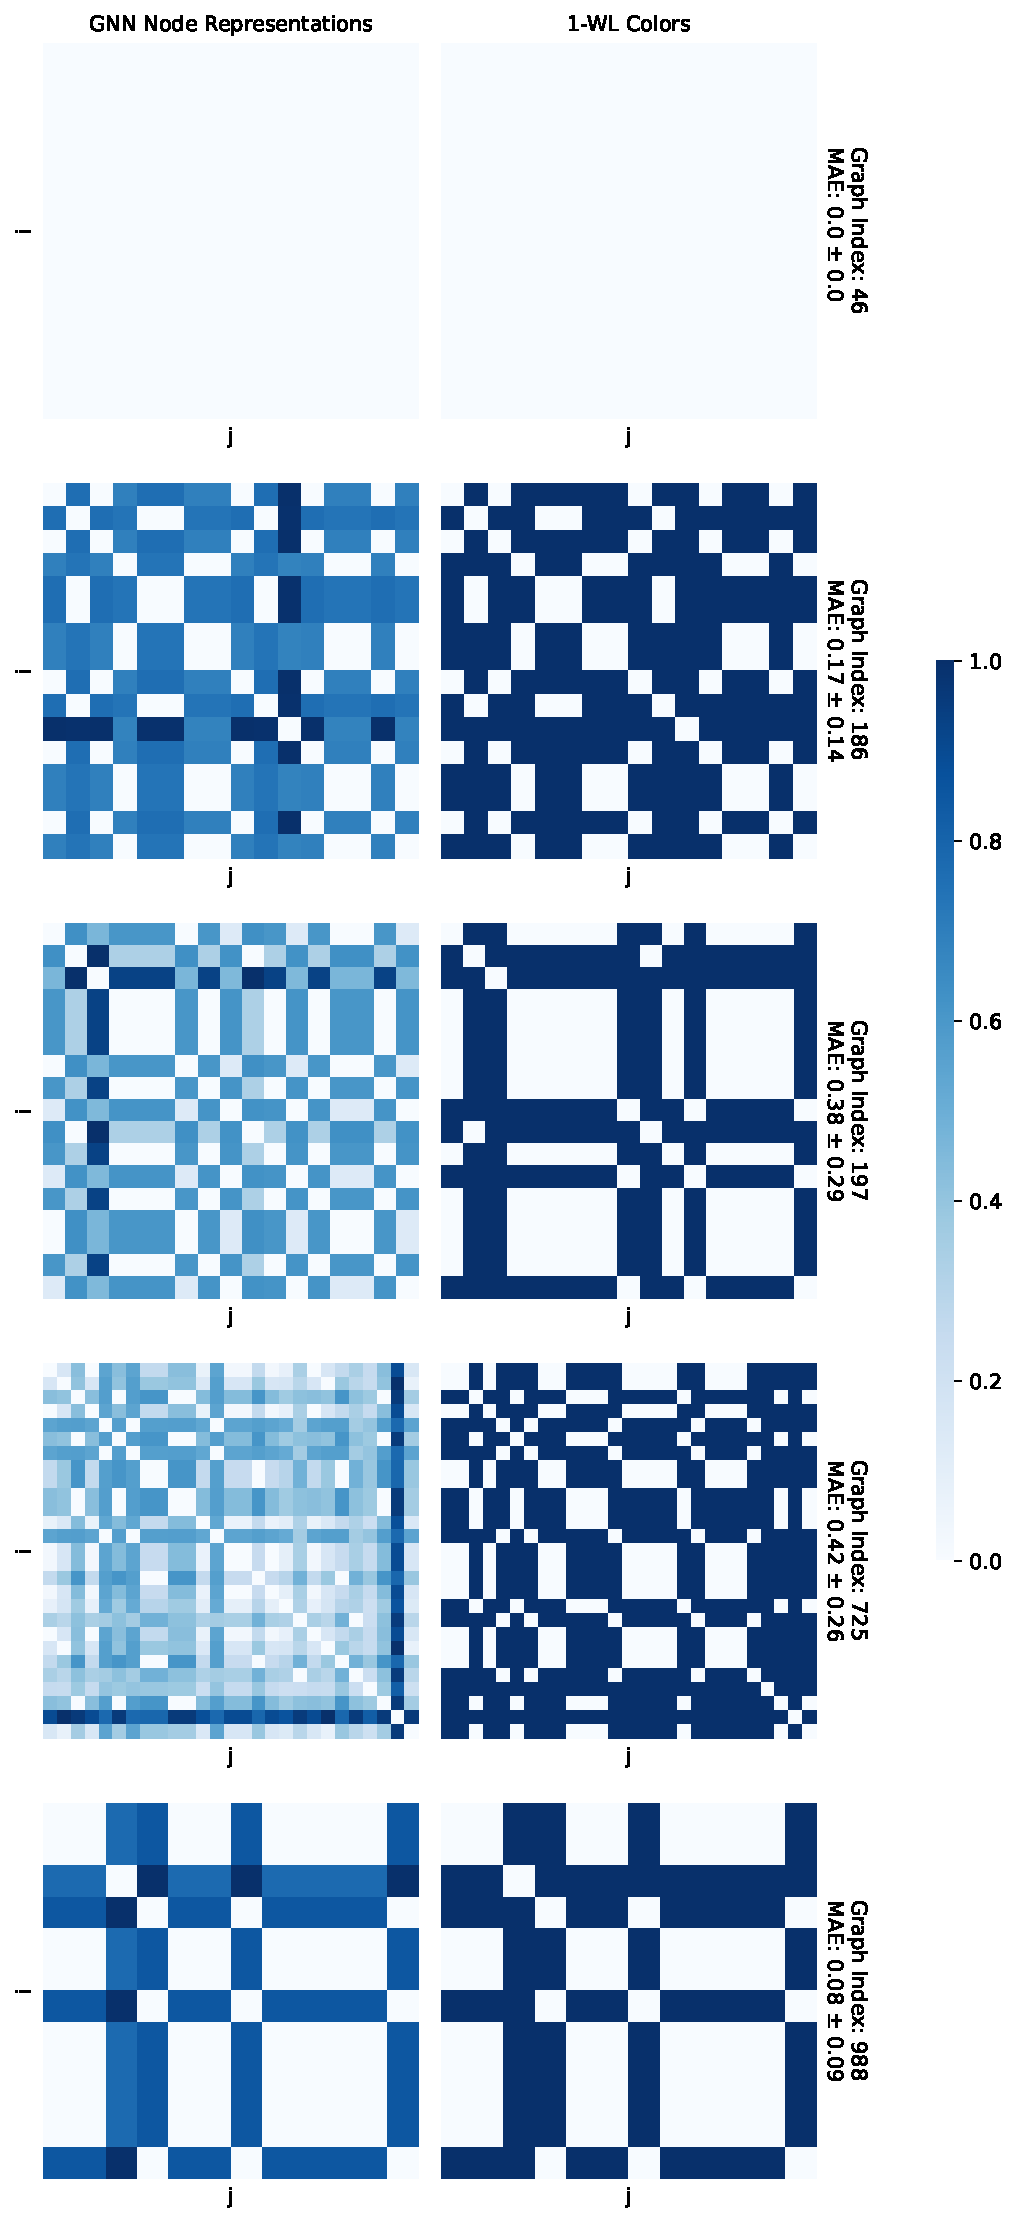
\includegraphics[width=\textwidth, right]{Figures/heatmaps_IMDB-BINARY_1.pdf}
    \end{minipage}
    \hfill
    \caption{Visualizing the performance of the best performing GNN on the \textsc{Imdb-Binary} dataset in approximating node colors computed by the 1-WL algorithm. The ten graphs shown are randomly sampled from the GNN's test set, and the 1-WL algorithm ran only for one iteration. The average error for the entire test set is $0.14 \pm 0.15$. \newline
    Note that \textsc{Imdb binary} does not contain any node features, so we artificially initialize each node feature with a one-hot encoding of its degree.}
    \label{fig:gnn_approx_imdb}
\end{figure}

\begin{figure}[!ht]
    \centering
    \begin{subfigure}[b]{0.45992852703\textwidth}
        \centering
        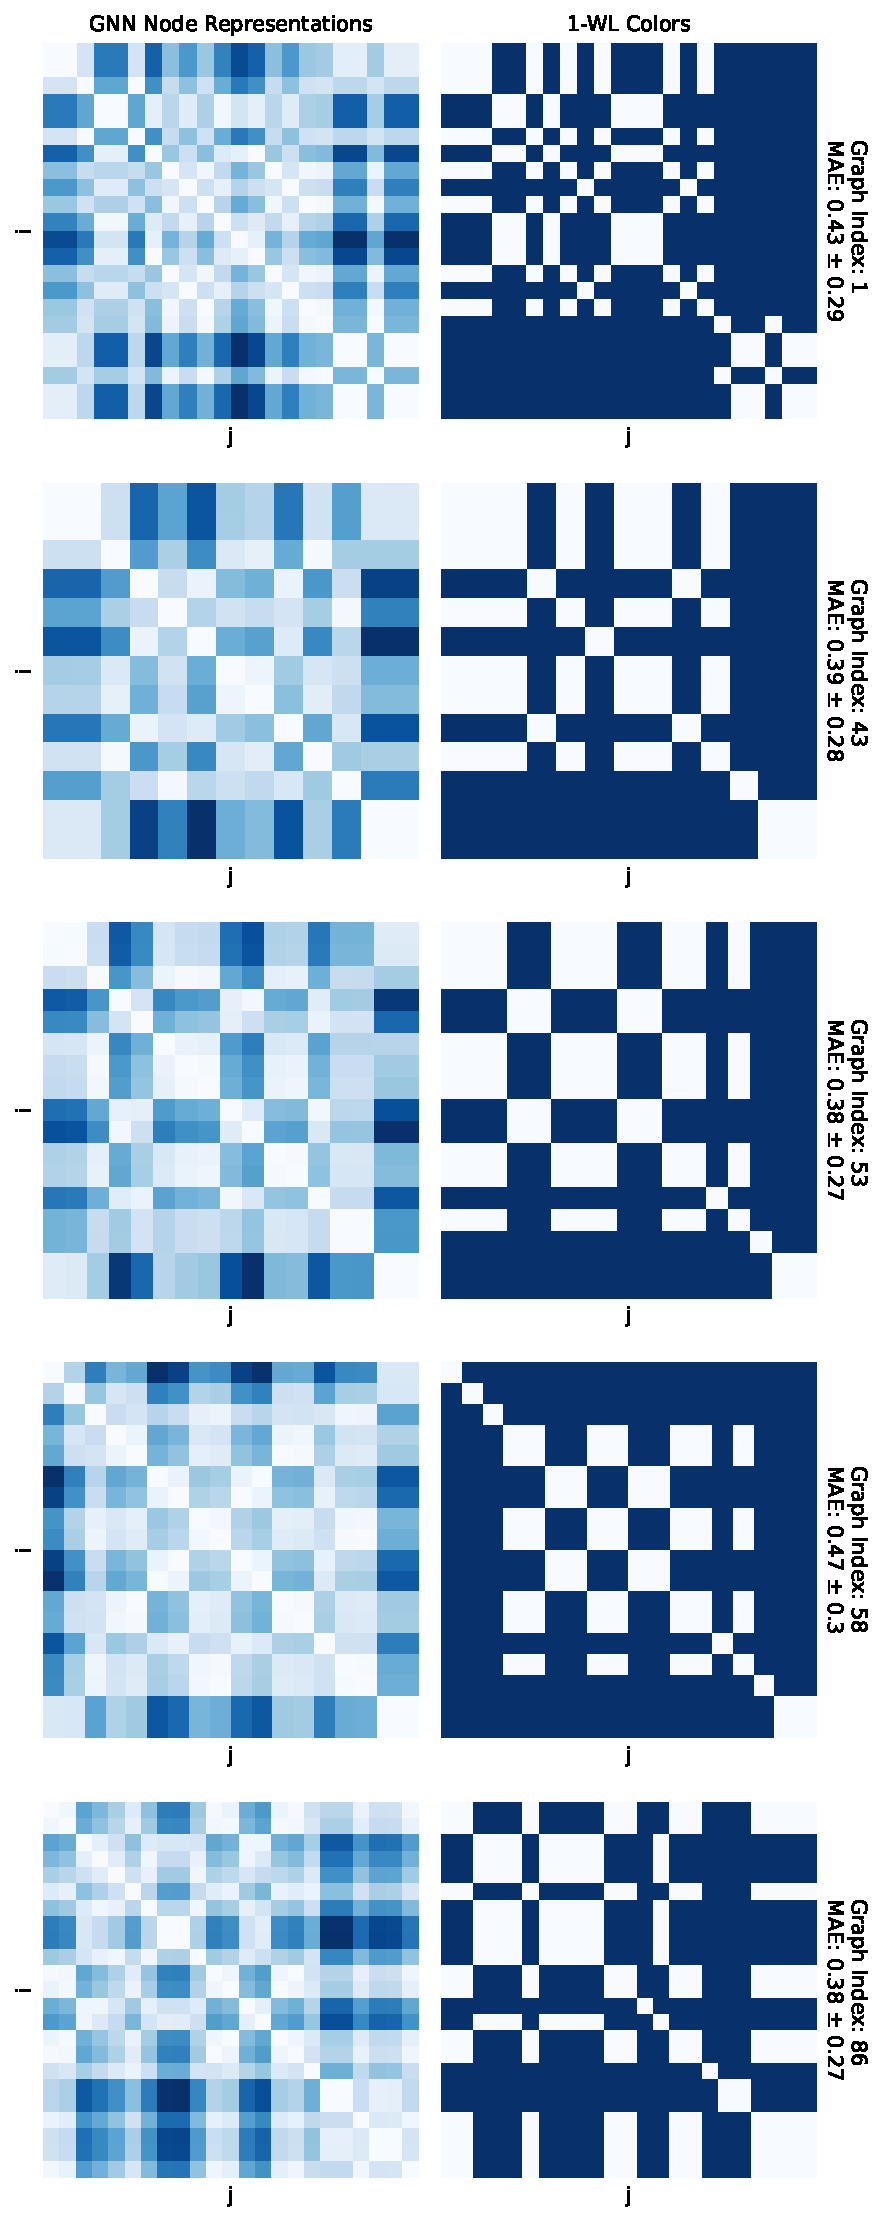
\includegraphics[width=\textwidth, left]{Figures/heatmaps_MUTAG_0.pdf}
    \end{subfigure}
    \hfill
    \begin{subfigure}[b]{0.53007147296\textwidth}
        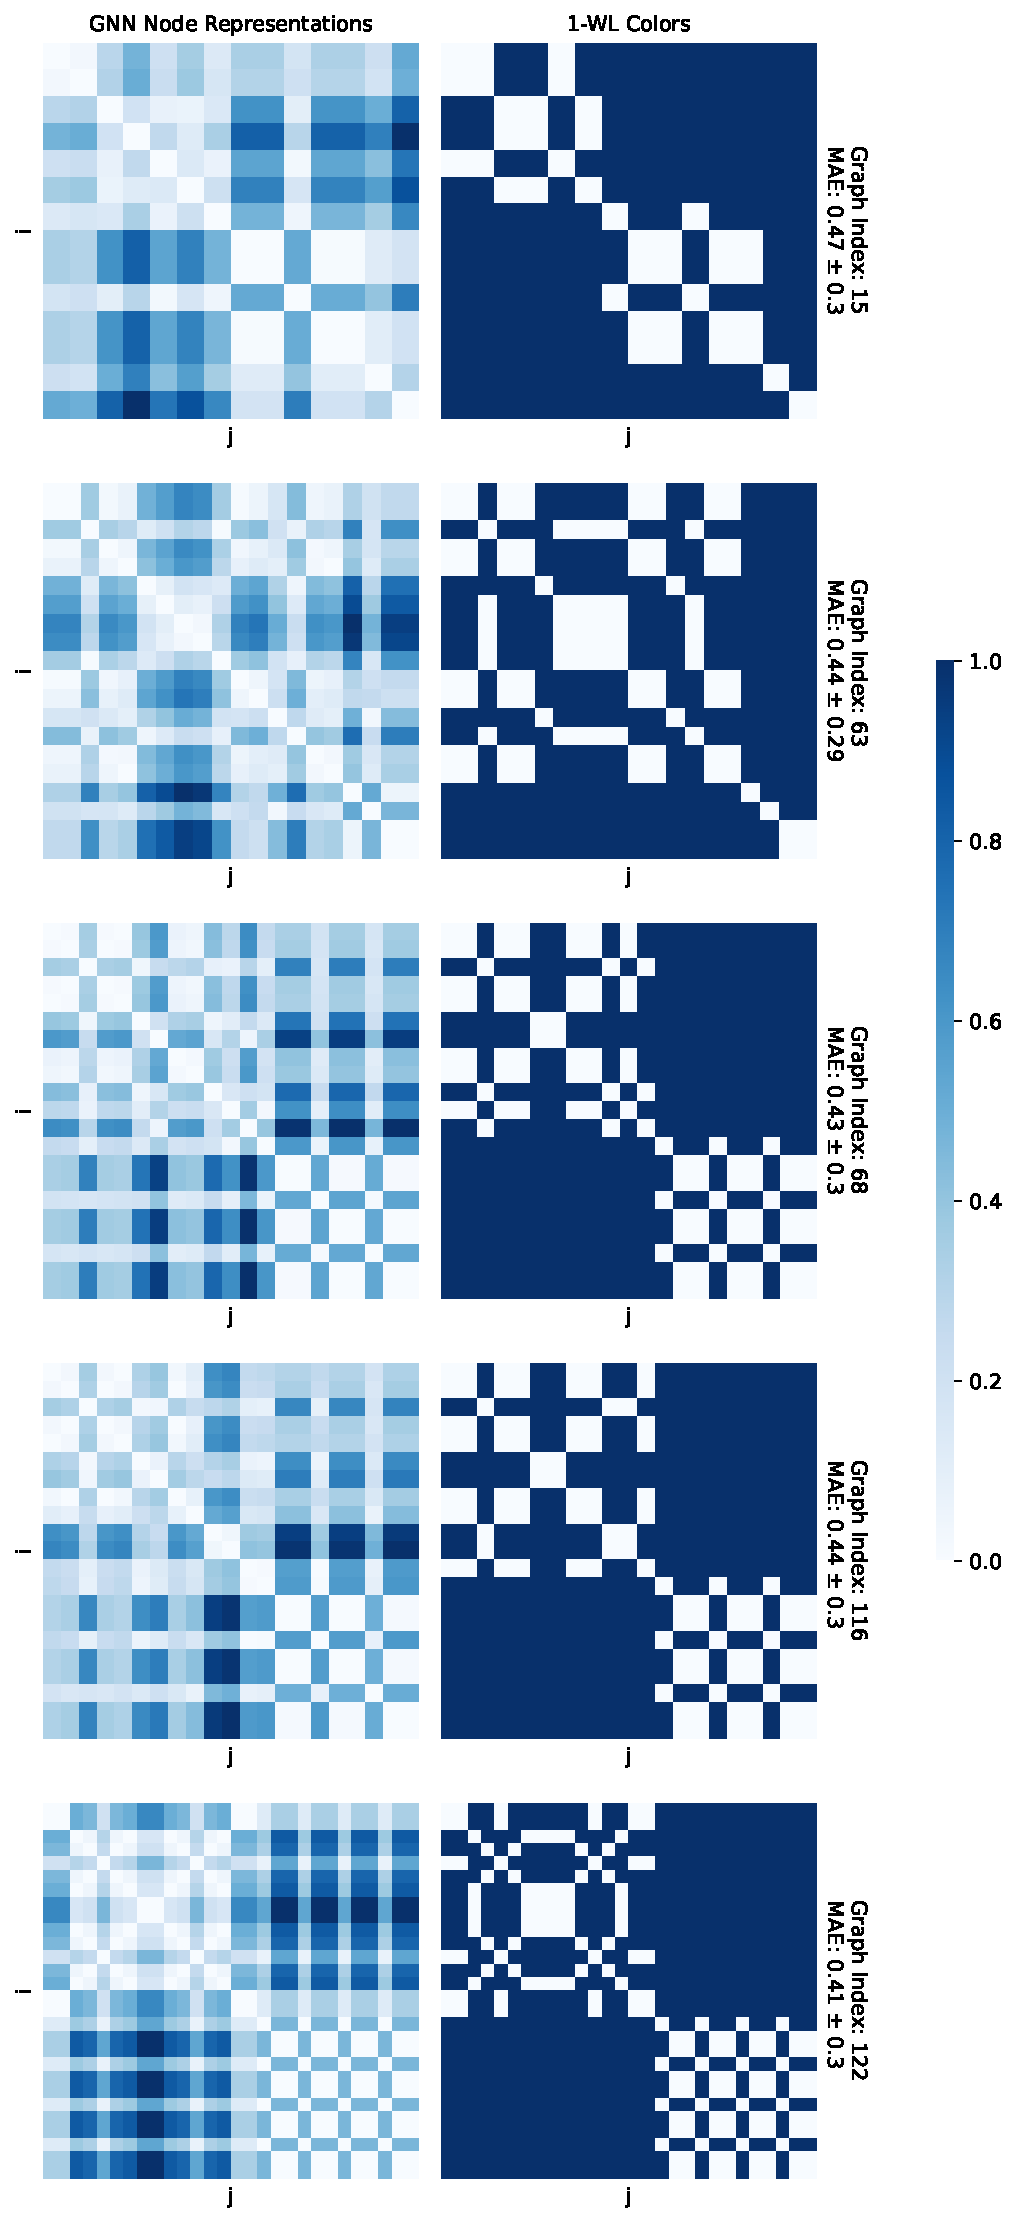
\includegraphics[width=\textwidth, right]{Figures/heatmaps_MUTAG_1.pdf}
    \end{subfigure}
    \hfill
    \caption{Visualizing the performance of the best performing GNN on the \textsc{Mutag} dataset in approximating node colors computed by the 1-WL algorithm. The ten graphs shown are randomly sampled from the GNN's test set, and the 1-WL algorithm ran only for three iteration. The average error for the entire test set is $0.42 \pm 0.29$.}
    \label{fig:gnn_approx_mutag}
\end{figure}

\begin{figure}[!ht]
    \centering
    \begin{minipage}[b]{0.45992852703\textwidth}
        \centering
        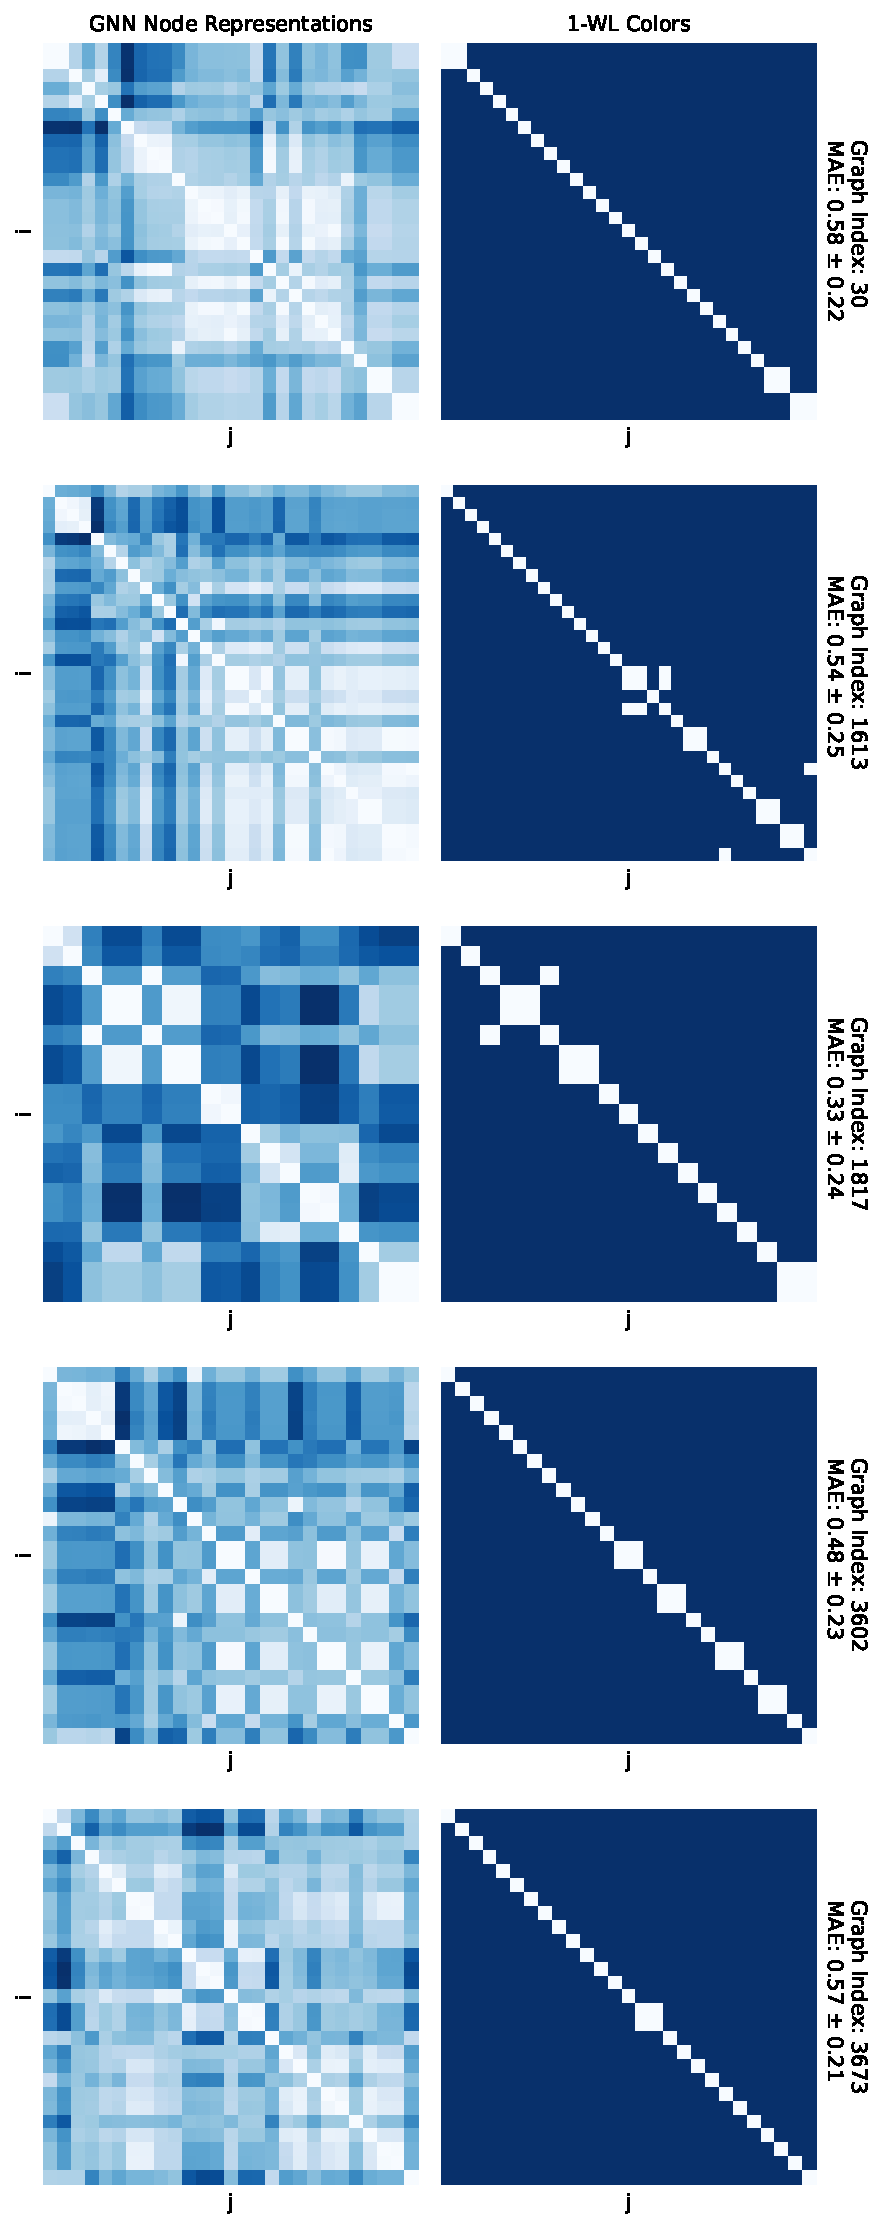
\includegraphics[width=\textwidth, left]{Figures/heatmaps_NCI1_0.pdf}
    \end{minipage}
    \hfill
    \begin{minipage}[b]{0.53007147296\textwidth}
        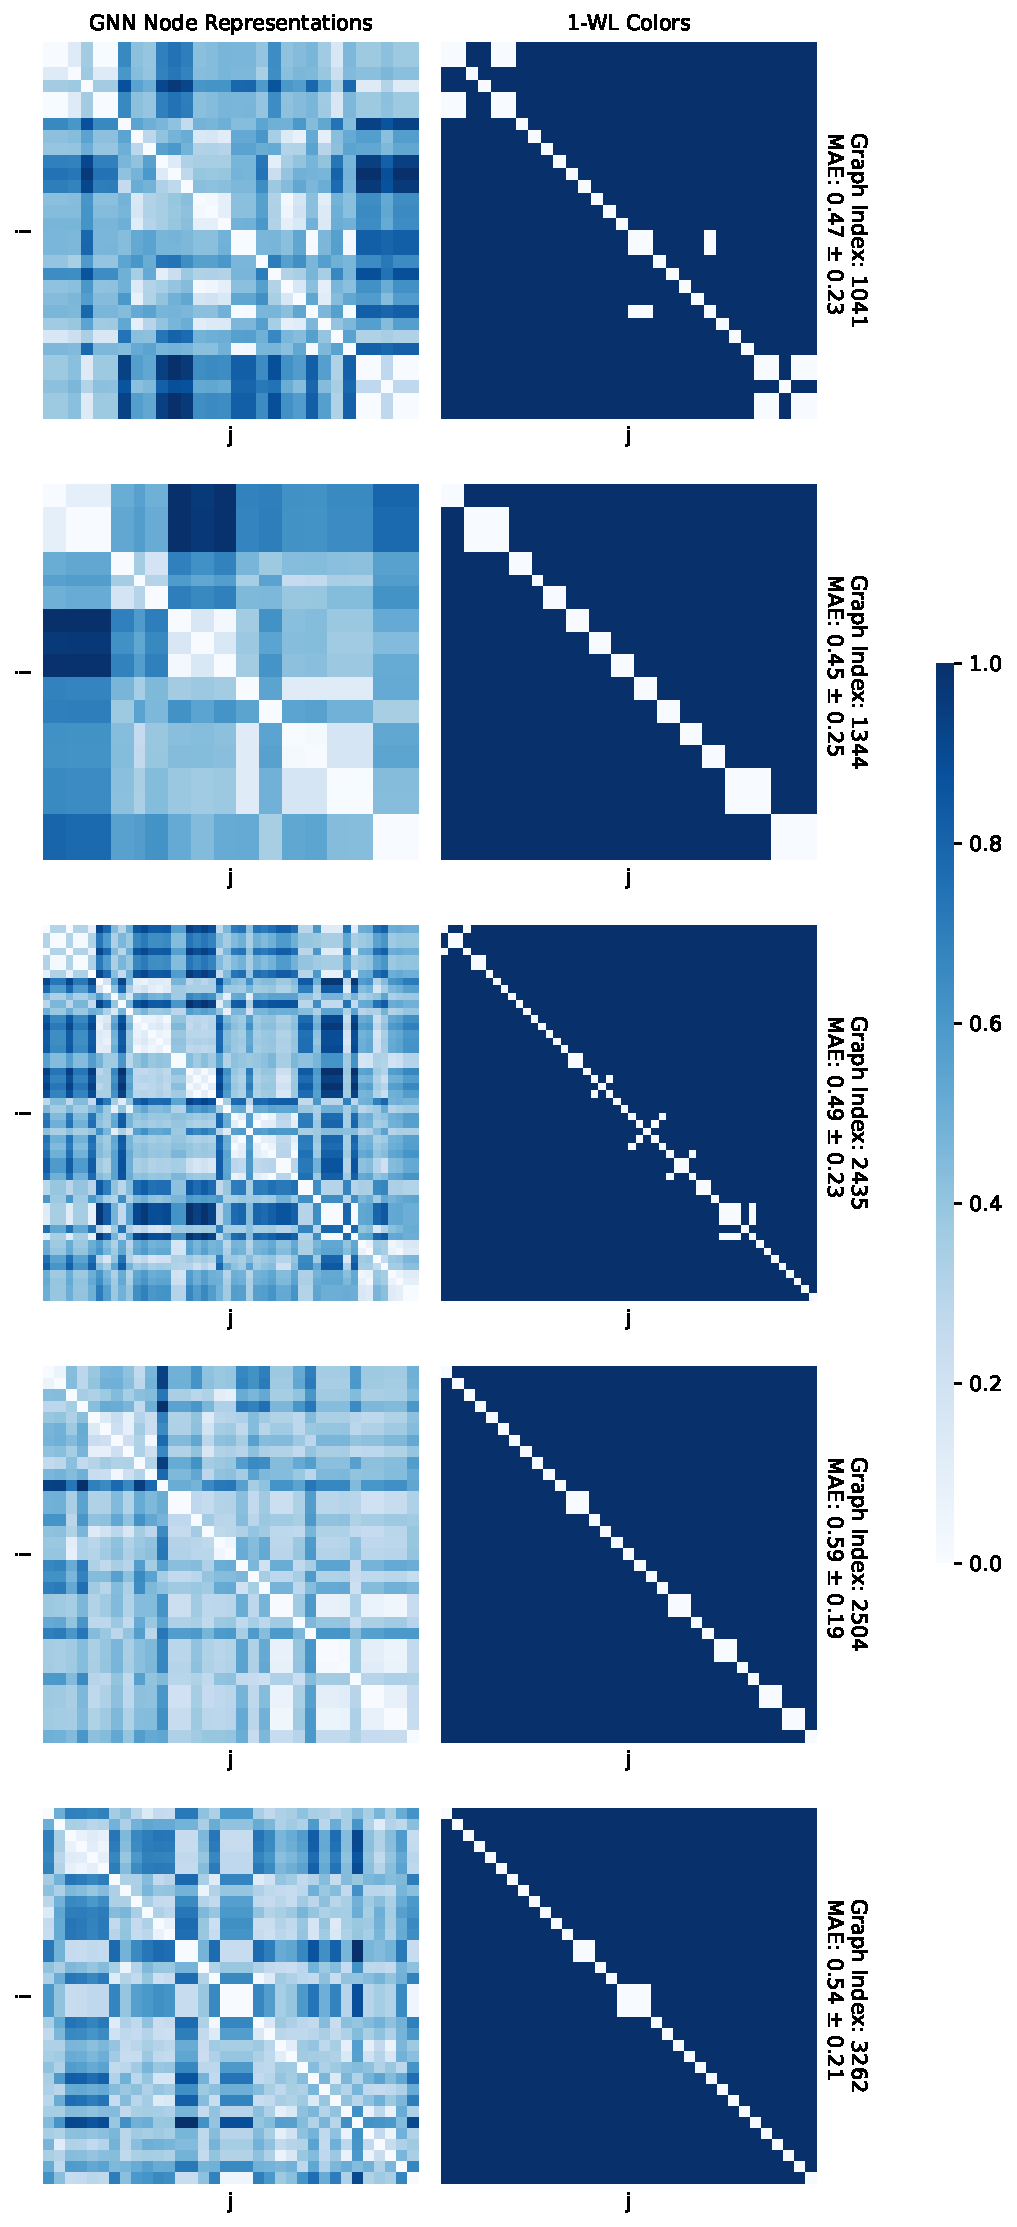
\includegraphics[width=\textwidth, right]{Figures/heatmaps_NCI1_1.pdf}
    \end{minipage}
    \hfill
    \caption{Visualizing the performance of the best performing GNN on the \textsc{Nci1} dataset in approximating node colors computed by the 1-WL algorithm. The ten graphs shown are randomly sampled from the GNN's test set, and the 1-WL algorithm ran only for three iteration. The average error for the entire test set is $0.50 \pm 0.24$.}
    \label{fig:gnn_approx_nci_3}
\end{figure}

\begin{figure}[!ht]
    \centering
    \begin{minipage}[b]{0.45992852703\textwidth}
        \centering
        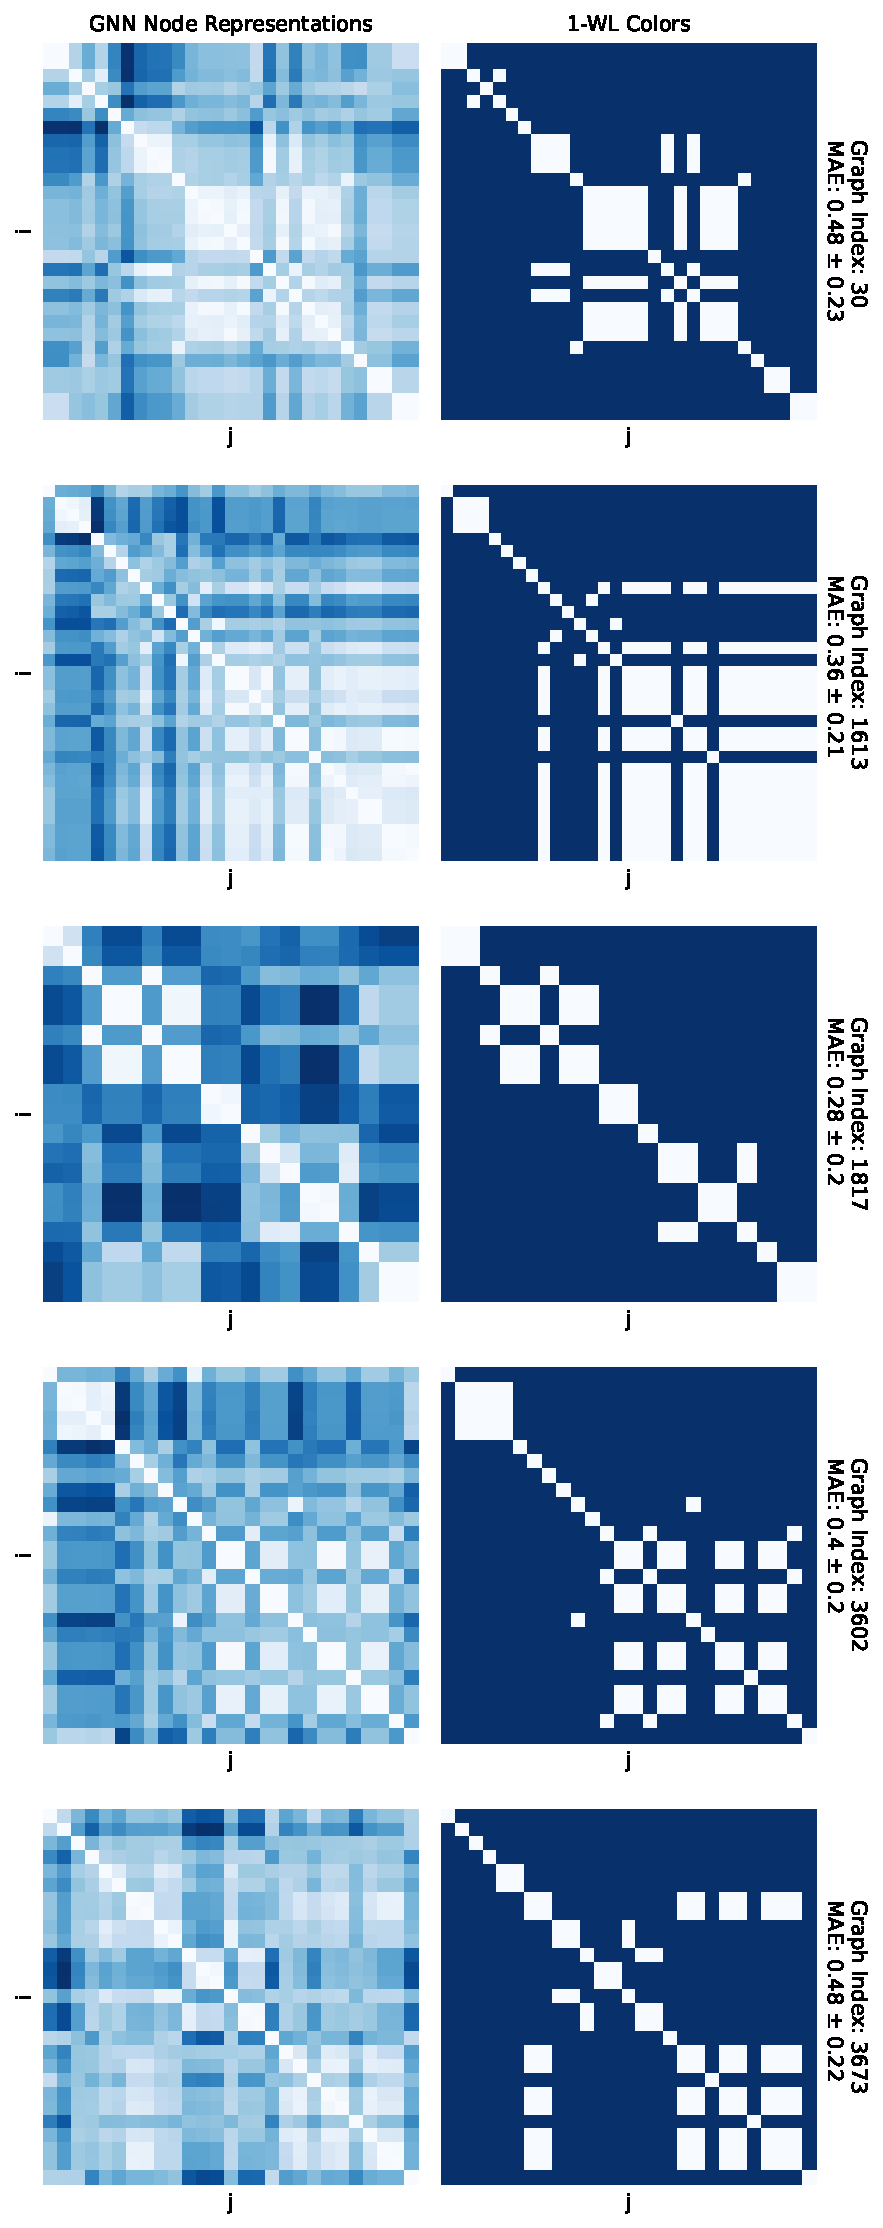
\includegraphics[width=\textwidth, left]{Figures/heatmaps_NCI1_0_k_wl_1.pdf}
    \end{minipage}
    \hfill
    \begin{minipage}[b]{0.53007147296\textwidth}
        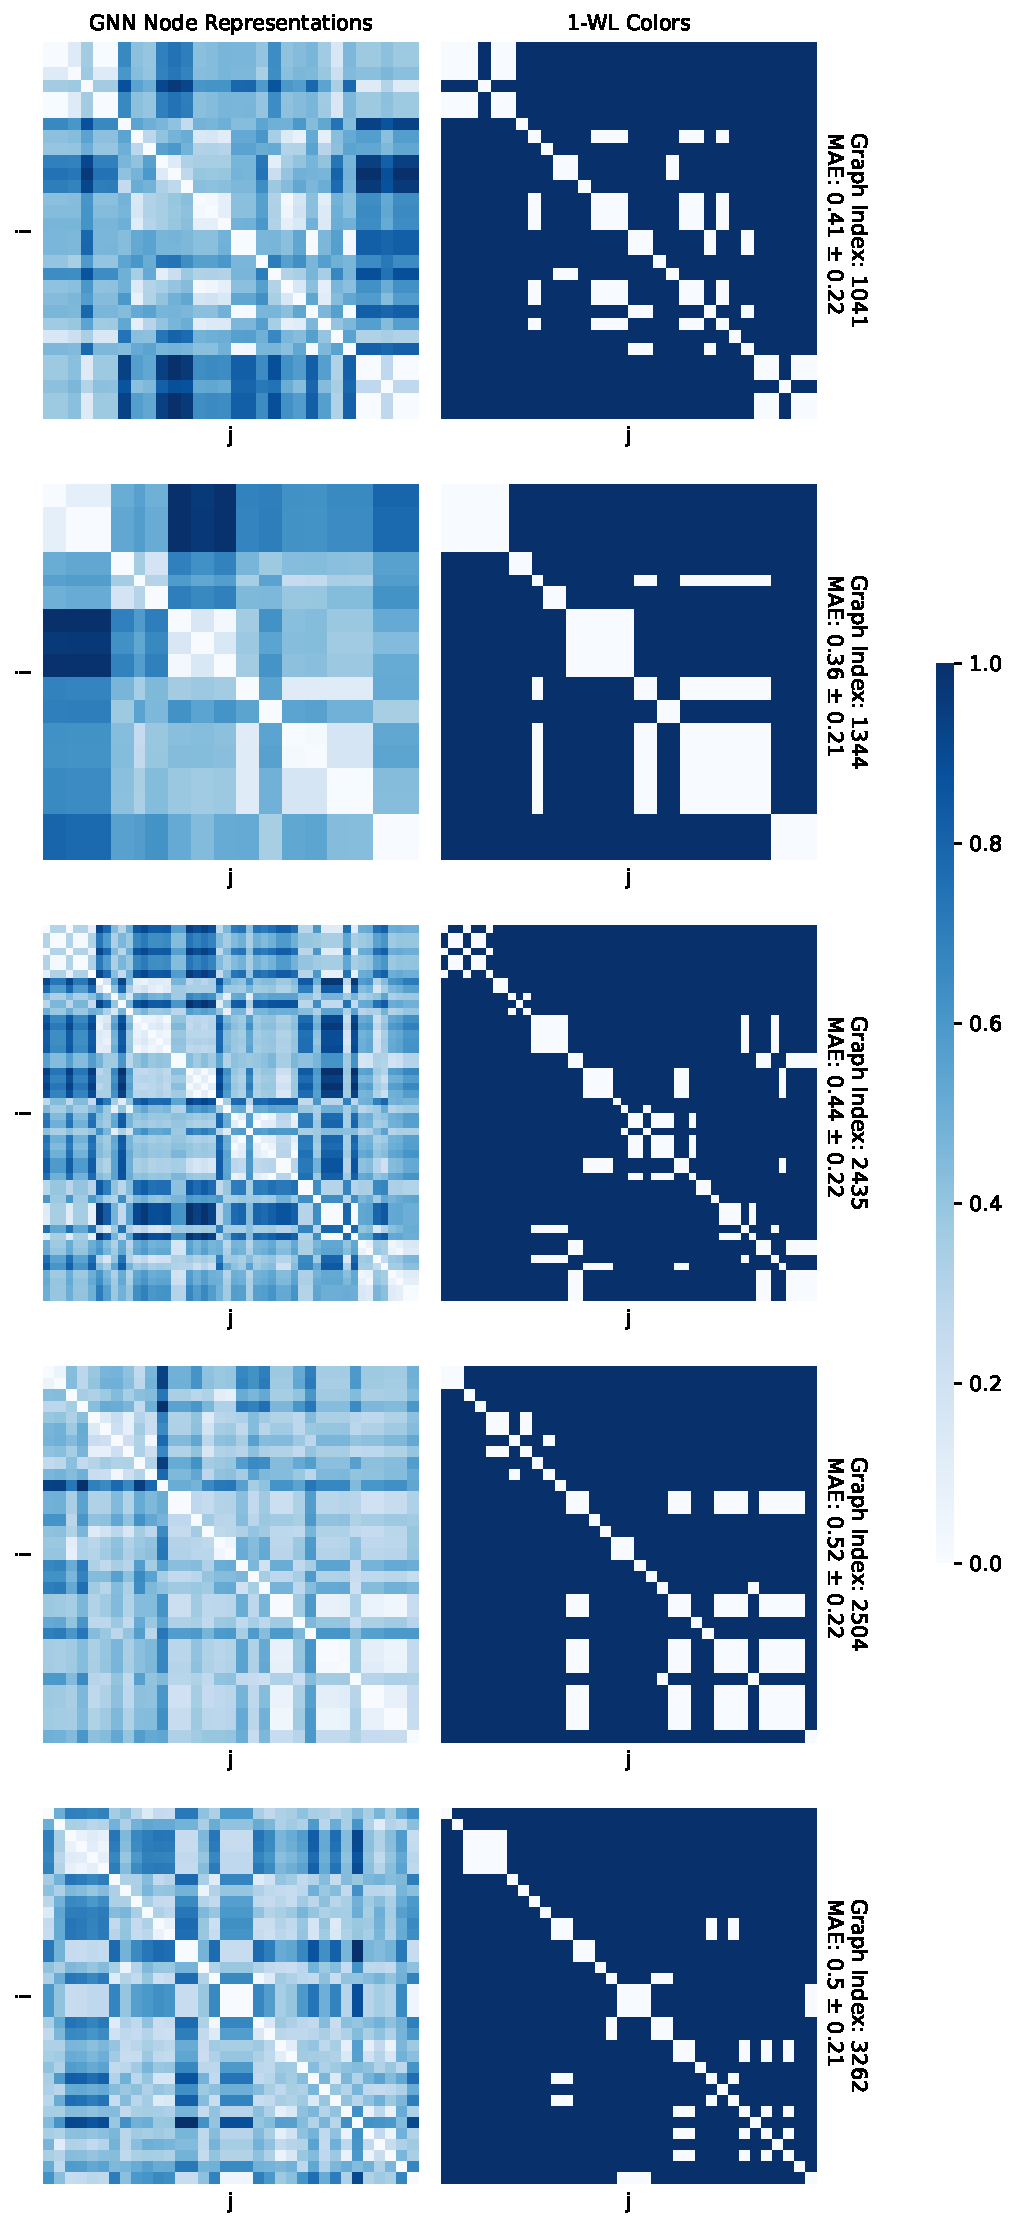
\includegraphics[width=\textwidth, right]{Figures/heatmaps_NCI1_1_k_wl_1.pdf}
    \end{minipage}
    \hfill
    \caption{Visualizing the performance of the best performing GNN on the \textsc{Nci1} dataset in approximating node colors computed by the 1-WL algorithm. The ten graphs shown are randomly sampled from the GNN's test set, and the 1-WL algorithm ran only for one iteration. The average error for the entire test set is $0.42 \pm 0.22$.}
    \label{fig:gnn_approx_nci_1}
\end{figure}

\begin{figure}[!ht]
    \centering
    \begin{minipage}[b]{0.45992852703\textwidth}
        \centering
        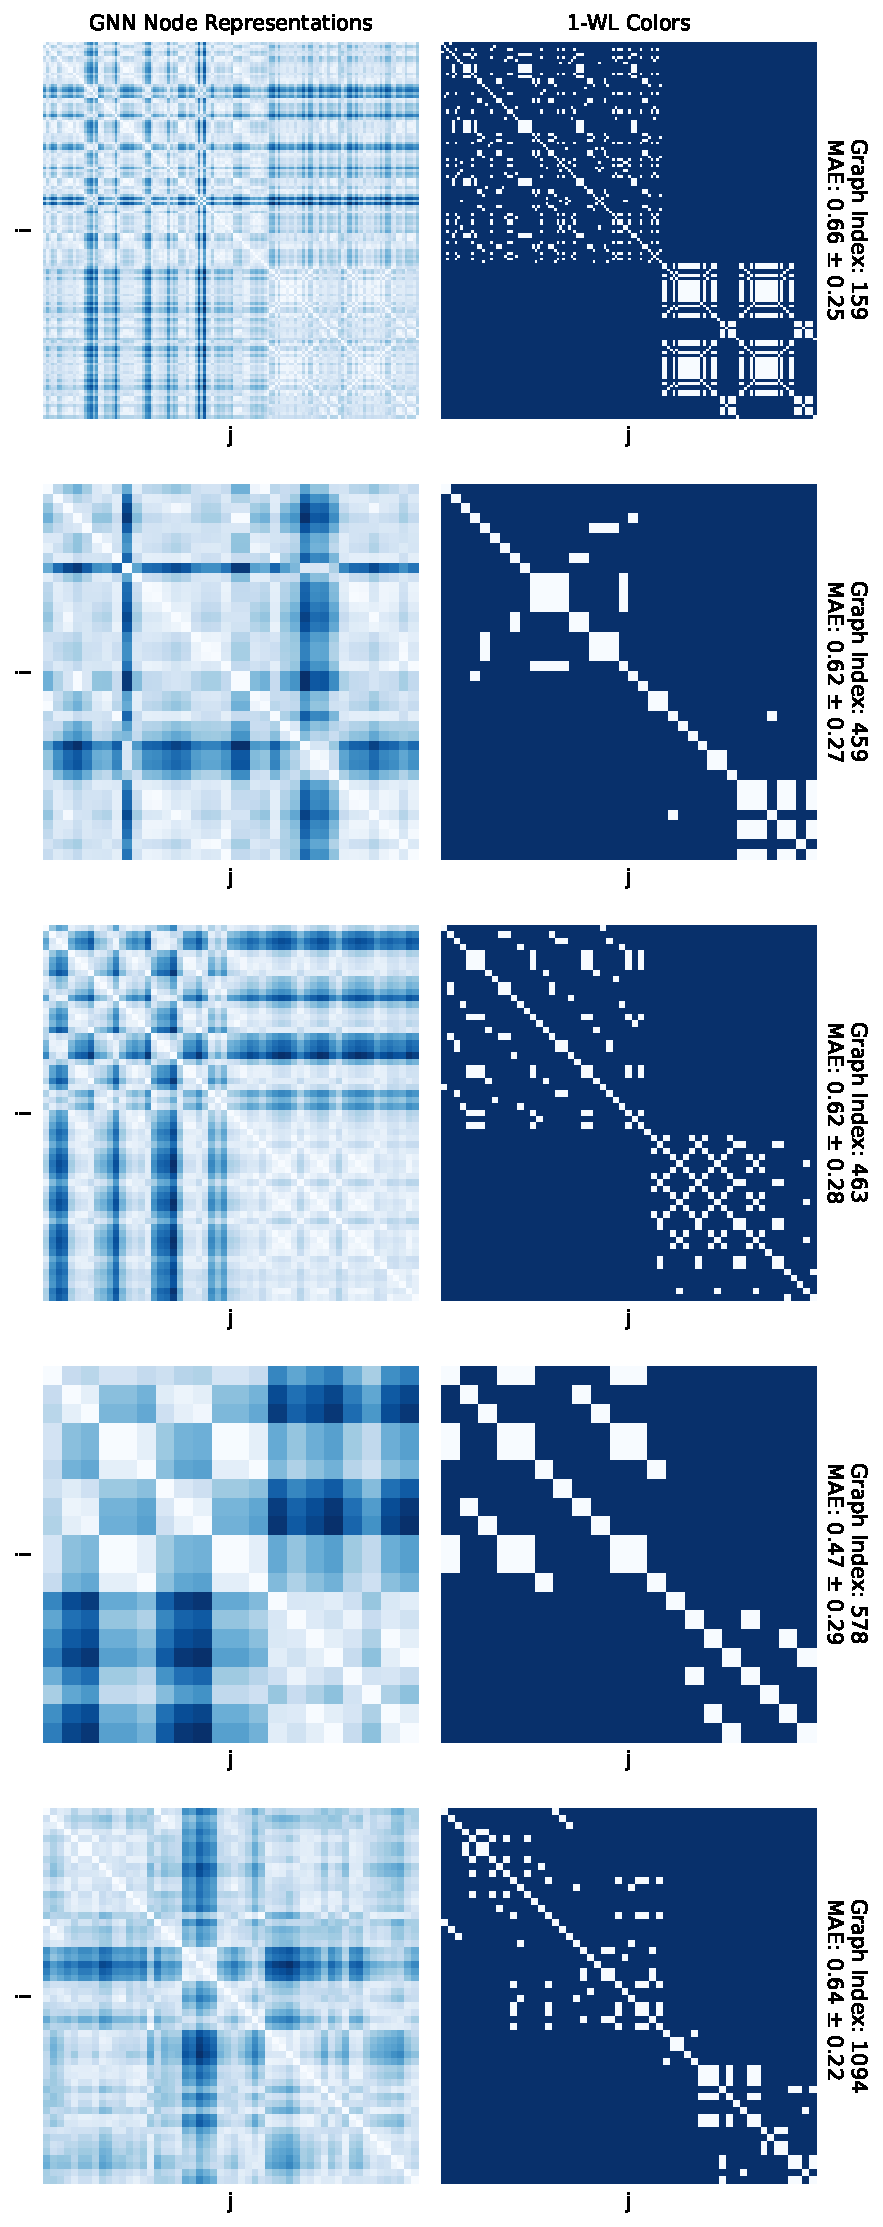
\includegraphics[width=\textwidth, left]{Figures/heatmaps_PROTEINS_0.pdf}
    \end{minipage}
    \hfill
    \begin{minipage}[b]{0.53007147296\textwidth}
        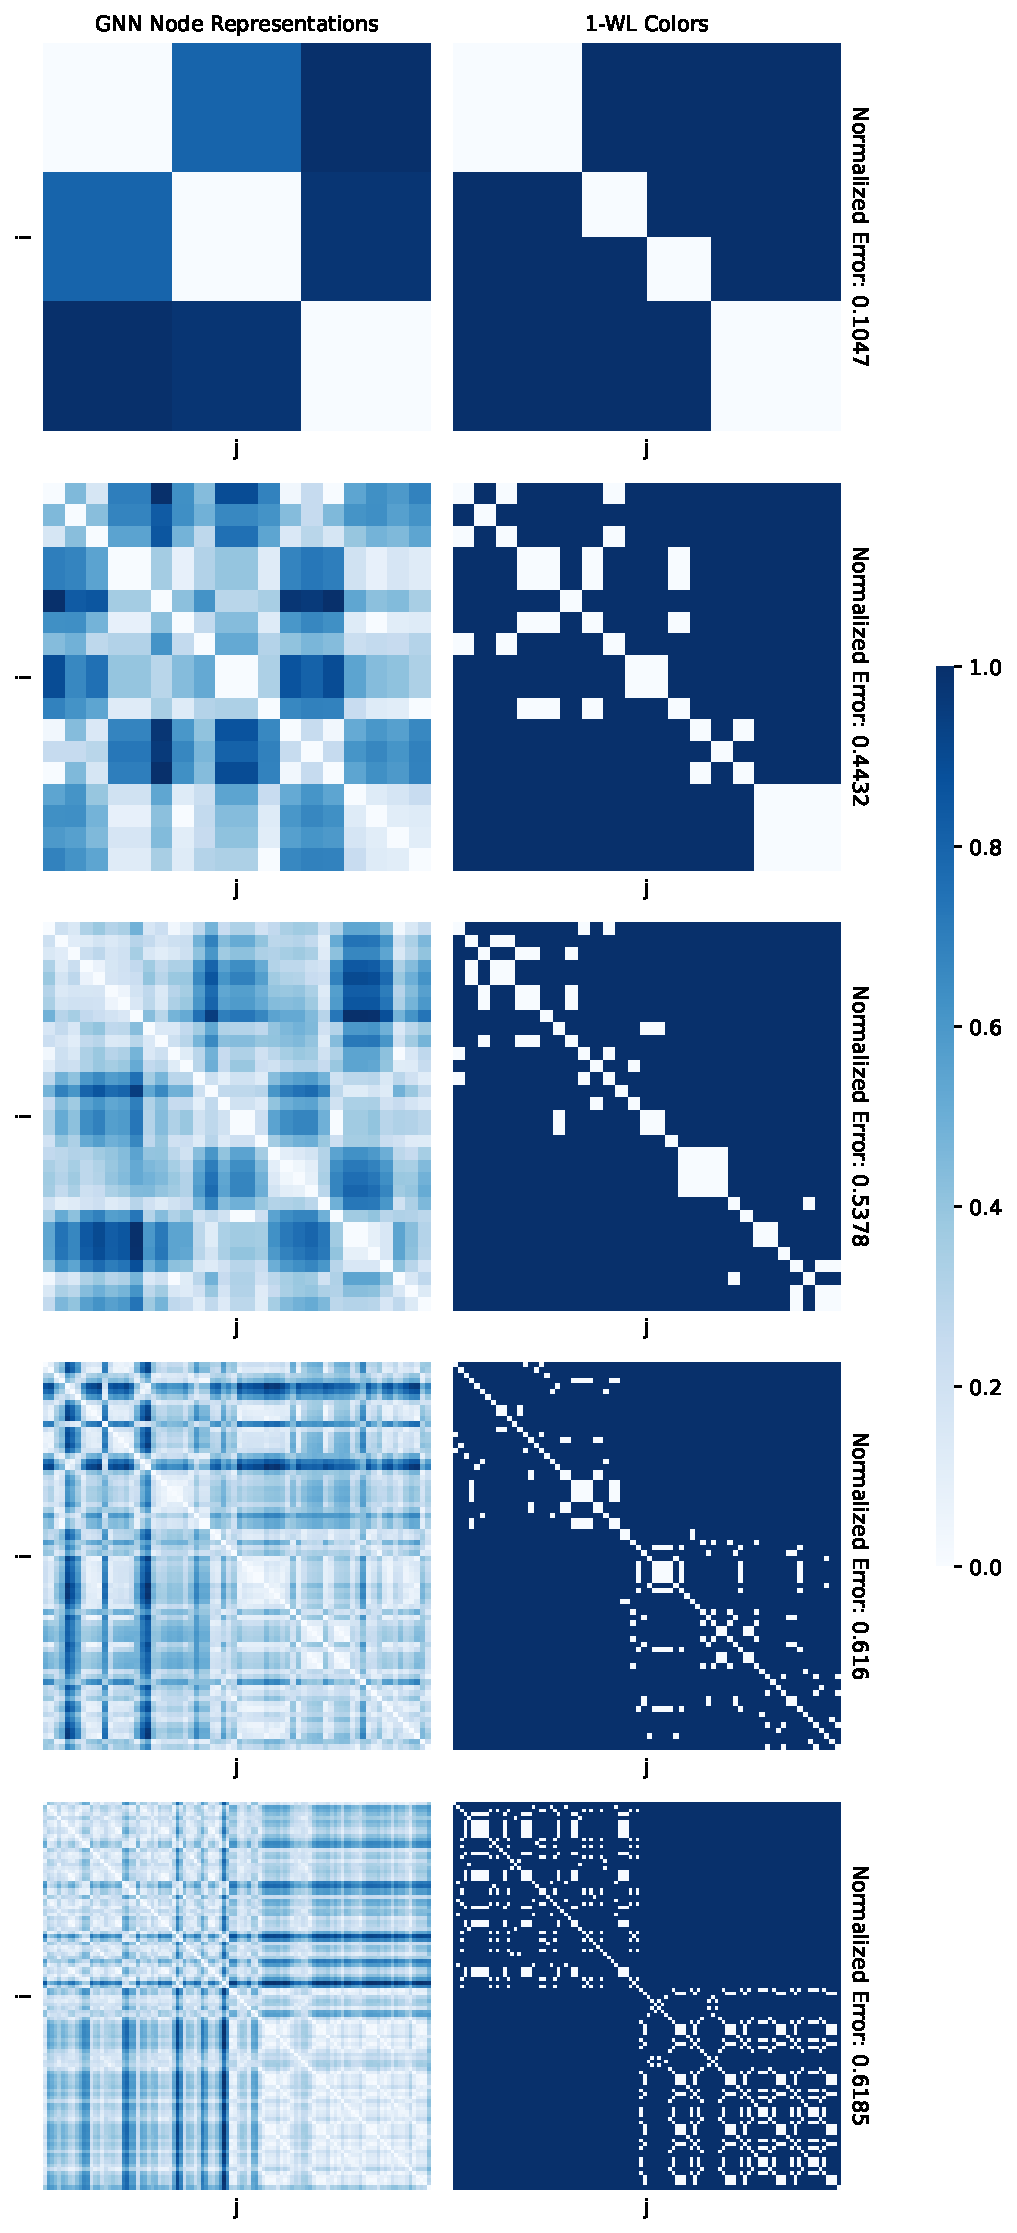
\includegraphics[width=\textwidth, right]{Figures/heatmaps_PROTEINS_1.pdf}
    \end{minipage}
    \hfill
    \caption{Visualizing the performance of the best performing GNN on the \textsc{Proteins} dataset in approximating node colors computed by the 1-WL algorithm. The ten graphs shown are randomly sampled from the GNN's test set, and the 1-WL algorithm ran only for one iteration. The average error for the entire test set is $0.49 \pm 0.26$.}
    \label{fig:gnn_approx_proteins}
\end{figure}

\begin{figure}[!ht]
    \centering
    \begin{minipage}[b]{0.45992852703\textwidth}
        \centering
        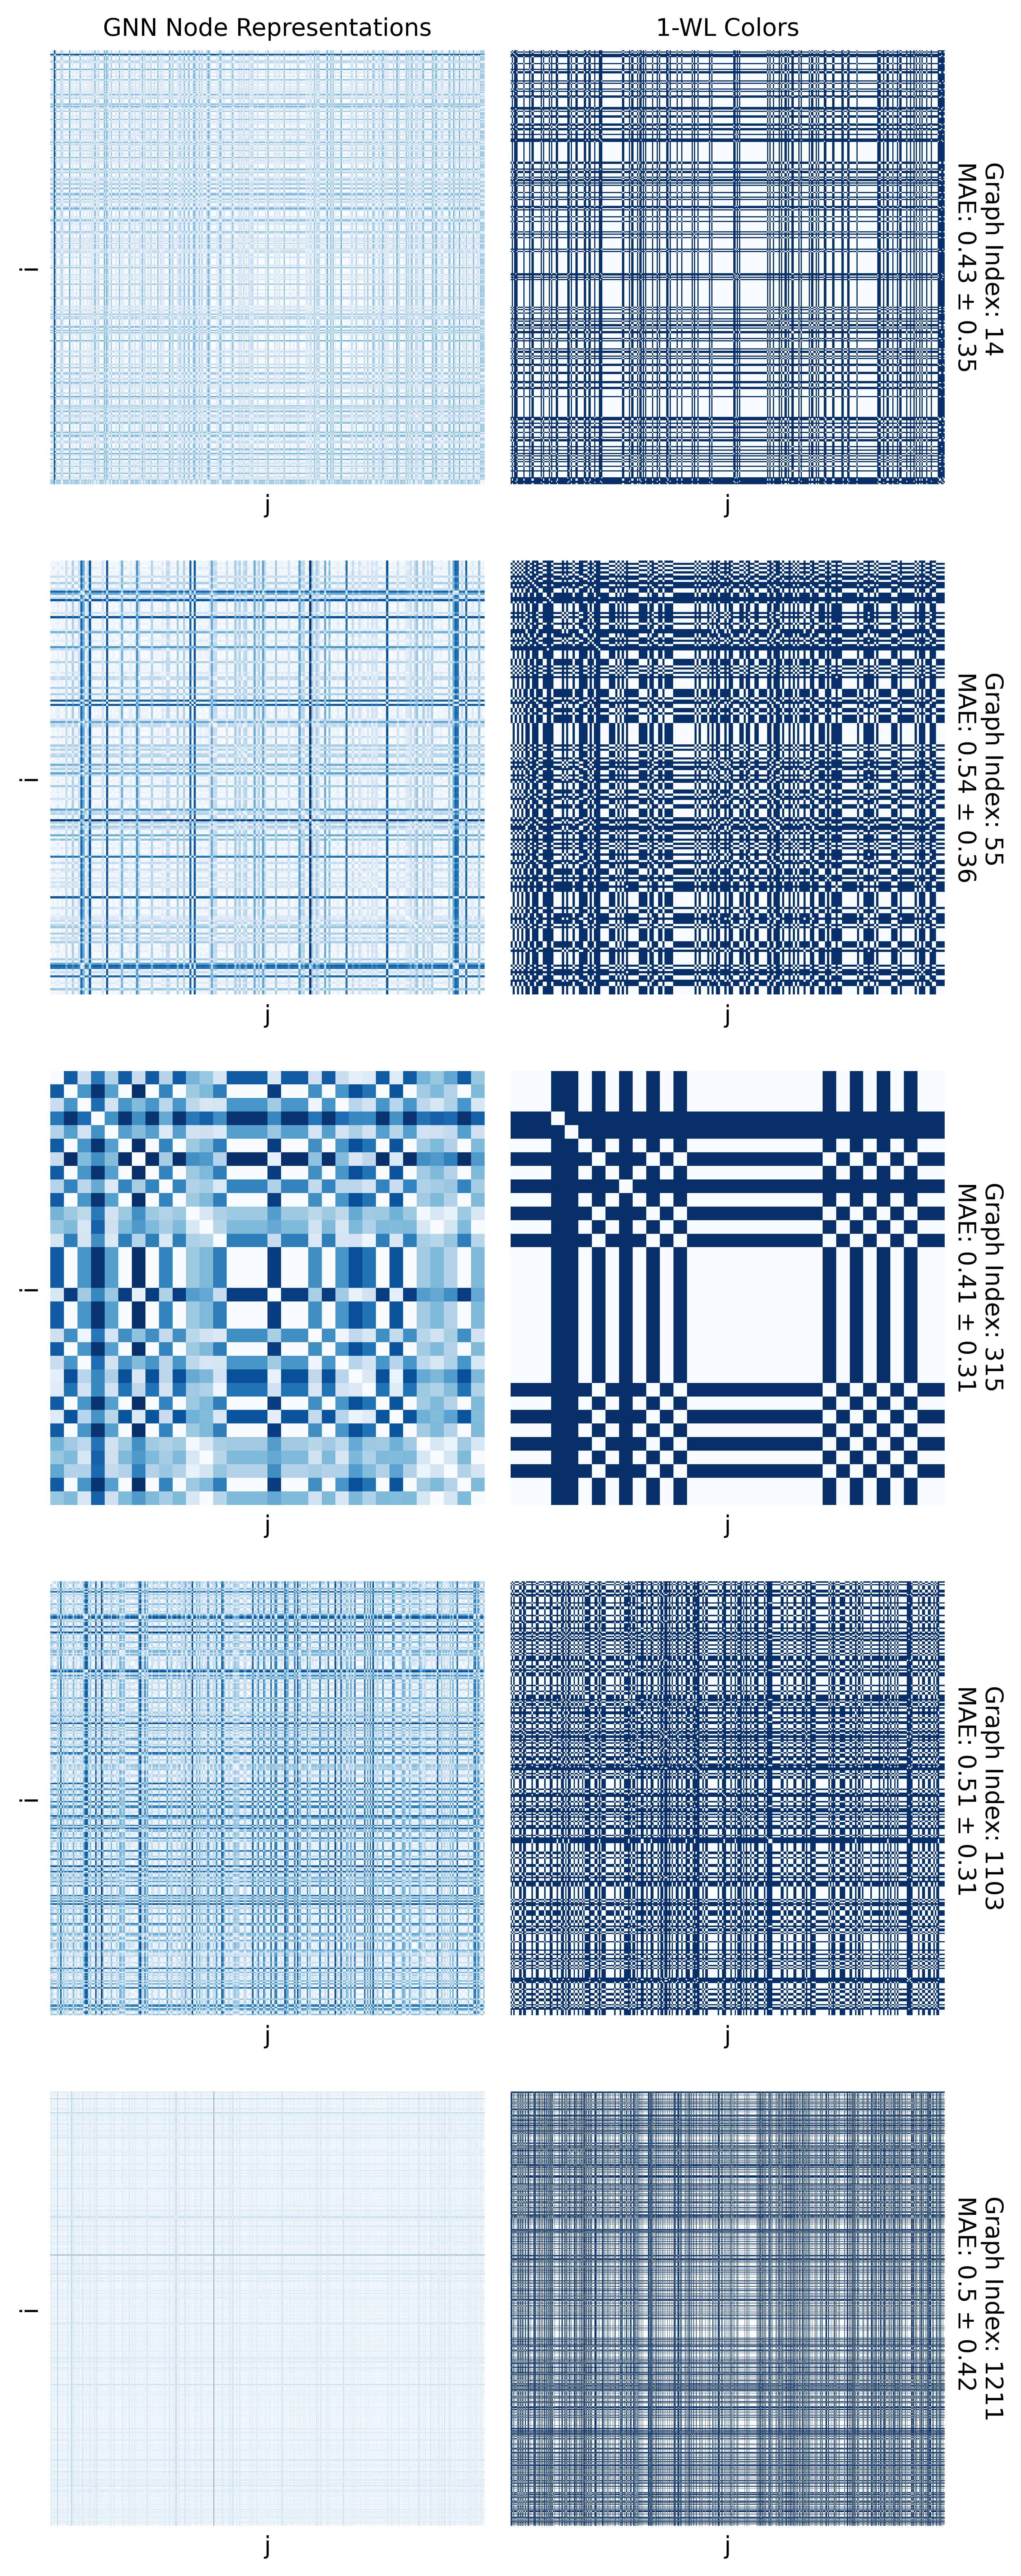
\includegraphics[width=\textwidth, left]{Figures/heatmaps_REDDIT-BINARY_0.png}
    \end{minipage}
    \hfill
    \begin{minipage}[b]{0.53007147296\textwidth}
        \includegraphics[width=\textwidth, right]{Figures/heatmaps_REDDIT-BINARY_1.png}
    \end{minipage}
    \hfill
    \caption{Visualizing the performance of the best performing GNN on the \reddit dataset in approximating node colors computed by the 1-WL algorithm. The ten graphs shown are randomly sampled from the GNN's test set, and the 1-WL algorithm ran only for one iteration. The average error for the entire test set is $0.48 \pm 0.32$.}
    \label{fig:gnn_approx_reddit}
\end{figure}